\lab{Data Visualization}{Data Visualization}
\label{lab:DataVis}
\objective{Correctly presenting and interpreting data with visualizations is both a science and an art.
% Indeed, effectively communicating complex relationships through data visualization is crucial to gaining the understanding needed to make important and difficult decisions.
In this lab we discuss and demonstrate the principles of good data visualization, including the key characteristics of good graphs, common mistakes, and how to avoid unethical visualizations.}


\section*{The Importance of Visualizations} % =================================

Visualizations of data often reveal insights that may not immediately obvious from simple statistics.
The following data set, known as \emph{Anscombe's quartet}, is a famous example of the importance of graphing data.

\begin{table}[H]
\small{
\begin{tabular}{rr|rr|rr|rr}
    \multicolumn{2}{c|}{I}    & \multicolumn{2}{|c|}{II} &
    \multicolumn{2}{|c|}{III} & \multicolumn{2}{|c}{IV} \\
    \multicolumn{1}{c}{$x$}   & \multicolumn{1}{c|}{$y$} &
    \multicolumn{1}{|c}{$x$}  & \multicolumn{1}{c|}{$y$} &
    \multicolumn{1}{|c}{$x$}  & \multicolumn{1}{c|}{$y$} &
    \multicolumn{1}{|c}{$x$}  & \multicolumn{1}{c}{$y$} \\
    \hline
    10.0 & 8.04  & 10.0 & 9.14 & 10.0 & 7.46  & 8.0  & 6.58  \\
    8.0  & 6.95  & 8.0  & 8.14 & 8.0  & 6.77  & 8.0  & 5.76  \\
    13.0 & 7.58  & 13.0 & 8.74 & 13.0 & 12.74 & 8.0  & 7.71  \\
    9.0  & 8.81  & 9.0  & 8.77 & 9.0  & 7.11  & 8.0  & 8.84  \\
    11.0 & 8.33  & 11.0 & 9.26 & 11.0 & 7.81  & 8.0  & 8.47  \\
    14.0 & 9.96  & 14.0 & 8.10 & 14.0 & 8.84  & 8.0  & 7.04  \\
    6.0  & 7.24  & 6.0  & 6.13 & 6.0  & 6.08  & 8.0  & 5.25  \\
    4.0  & 4.26  & 4.0  & 3.10 & 4.0  & 5.39  & 19.0 & 12.50 \\
    12.0 & 10.84 & 12.0 & 9.13 & 12.0 & 8.15  & 8.0  & 5.56  \\
    7.0  & 4.82  & 7.0  & 7.26 & 7.0  & 6.42  & 8.0  & 7.91  \\
    5.0  & 5.68  & 5.0  & 4.74 & 5.0  & 5.73  & 8.0  & 6.89  \\
\end{tabular}}
\end{table}

Each section of Anscombe's quartet shares the following statistical properties:
\begin{itemize}
\setlength\itemsep{0em}
    \item The means are $9$ for $x$ and $7.5$ for $y$.
    \item The sample variances are $11$ for $x$ and $3.75$ for $y$.
    \item The correlation between $x$ and $y$ is $.816$.
    \item The linear least squares regression line is $y=\frac{1}{2}x+3$.
\end{itemize}

Despite these similarities, each section is quite different from the others.

\begin{problem} % Describe Anscombe's quartet.
The file \texttt{anscombe.npy} contains Anscombe's quartet in the same format as displayed above.
Plot each section of the quartet separately as a scatter plot.
Also plot the regression line $y = \frac{1}{2}x + 3$ on the domain $x\in[0,20]$ over each scatter plot.

Write a few sentences describing what makes each section unique.
\label{prob:anscombes-quartet}
\end{problem}

\section*{Principles of Good Data Visualization} % ============================

Effectively visualizing data involves technical expertise combined with design knowledge.
No visualization is perfect, but every good visualization must contains the following essential elements.

\begin{enumerate}
    \item \textbf{Clarity}.
    Visualizations should be self-explanatory.
    Always use specific titles and axis labels, and include units of measure.
    Use a legend or annotations where appropriate.

    \item \textbf{Simplicity}.
    A good visualization communicates everything that it needs to, but nothing more.
    Remove unnecessary or distracting elements of a graph, including 3-D effects or overly flashy colors.

    \item \textbf{Integrity}.
    Tell the truth, the whole truth, and nothing but the truth.
    It is almost always very easy to manipulate a visualization so that it supports a desired interpretation.
    Resist the temptation to morph a visualization into something that misrepresents the true nature of the data, even though that misrepresentation might support your hypotheses about the data.

    Every visualization should be presented together with information on who created it, where the data was obtained, how it was collected, whether it was cleaned or transformed, and whether there are conflicts of interest or possible biases present.
    Cite your sources.
\end{enumerate}

This list could be expanded, but virtually every good data visualization principle fits into these three categories in one way or another.

\section*{Improving Specific Types of Visualizations} % =======================

Data can be visualized in many forms and styles.
However, Most data sets are more naturally described with one type of visualization than another.
In the following sections, we explore how the plots we commonly use can be improved and refined.

\subsection*{Line Plots} % ----------------------------------------------------

A line plot connects ordered $(x,y)$ points with straight lines, and is therefore best for visualizing one or two ordered arrays, such as functional outputs over an ordered domain or a sequence of values over time.

When creating a line plot, consider the following details.
%
\begin{itemize}
    \item What do the axes represent? How should they be labeled?
    \item Would a linear scale or a logarithmic scale most clearly reveal patterns?
    \item What should the window limits be?
    \item Is the line an appropriate thickness and color?
    \item Should each point be distinctly marked, or is a smooth line preferable?
    \item Should multiple lines be in the same plot, or in separate subplots?
\end{itemize}

The \emph{Chebyshev polynomials} are a family of orthogonal polynomials that are recursively defined as follows.
\[T_0(x) = 1 \qquad T_1(x) = x \qquad\qquad T_{n+1} = 2xT_n(x) - T_{n-1}(x)\]
NumPy's \li{polynomial} module has a convenient tool for constructing these and other important polynomials.%
\footnote{\li{numpy.polynomial} also has tools for computing other polynomial families, including the Legendre, Hermite, and Laguerre polynomials.}
However, plotting several the polynomials on top of each other, especially with a legend, results in a very cluttered visual.

\begin{lstlisting}
>>> import numpy as np
>>> from matplotlib import pyplot as plt
>>> % matplotlib inline                     # Display notebook plots inline.

# Plot the first 9 Chebyshev polynomials in the same plot.
>>> T = np.polynomial.Chebyshev.basis
>>> x = np.linspace(-1, 1, 200)
>>> for n in range(9):
...     plt.plot(x, T(n)(x), label="n = "+str(n))
...
>>> plt.axis([-1.1, 1.1, -1.1, 1.1])        # Set the window limits.
>>> plt.legend()
\end{lstlisting}

\begin{figure}[H] % Chebyshev polynomials (bad example).
    \centering
    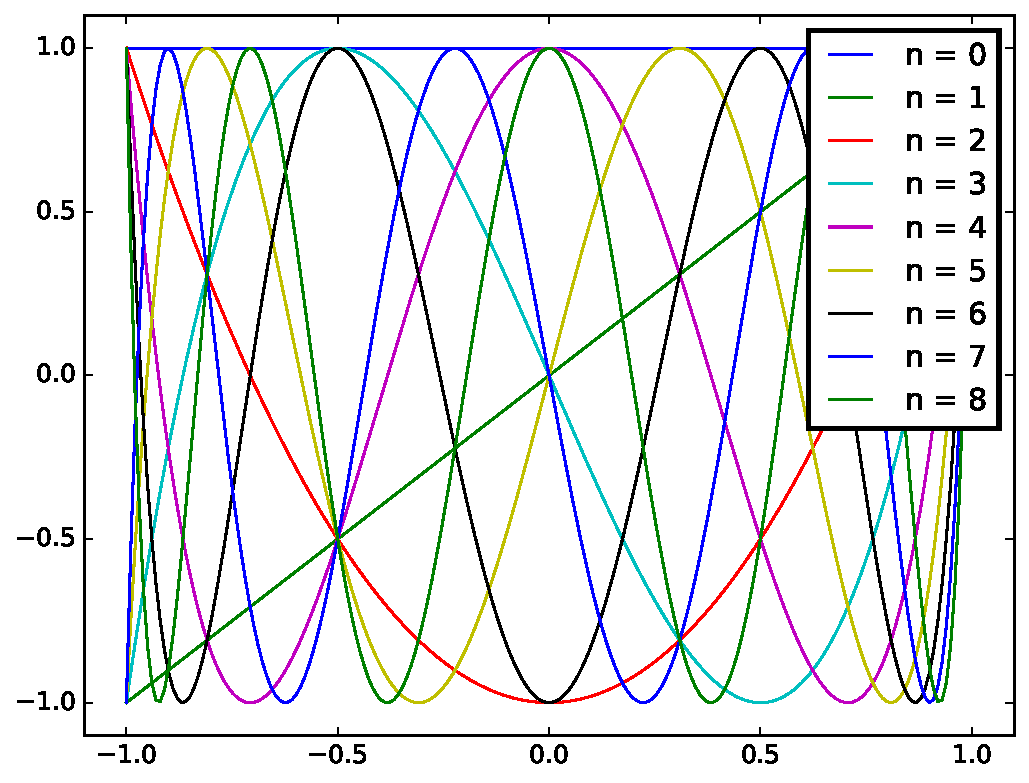
\includegraphics[width=.7\linewidth]{figures/chebyshev_bad.pdf}
\end{figure}

\newpage

This line plot can be improved in several easy ways.
%
\begin{enumerate}
    \item
    Use subplots to split the visualization into smaller, comparable pieces.
    Instead of using a legend, give each subplot a title.
    This method, called \emph{small multiples}, was made famous by Edward Tufte.
    \item Increase the line thicknesses to 2 or 3 (the default is 1).
    \item Remove extra tick marks and axis labels.
\end{enumerate}

Matplotlib's \li{plt.tick_params()}, summarized below, controls which tick marks and labels are displayed.
%
\begin{table}[H]
\begin{tabular}{r|c|l}
    Argument & Options & Description
    \\ \hline
    \li{axis} & \li{'x'}, \li{'y'}, \li{"both"} & Axis on which to operate. \\
    \li{which} & \li{"major"}, \li{"minor"}, \li{"both"} & Operate on major or minor ticks.\\
    \li{color} & Any Matplotlib color & Tick color. \\
    \li{labelcolor} & Any Matplotlib color & Tick label color. \\
    \li{bottom}, \li{top}, \li{left}, \li{right} & \li{"on"}, \li{"off"} & Turn ticks on or off. \\
    \li{labelbottom}, \li{labeltop}, & \li{"on"}, \li{"off"} & Turn tick labels on or off. \\
    \li{labelleft}, \li{labelright} & &
\end{tabular}
\end{table}

\begin{lstlisting}
>>> for n in range(9):
...     plt.subplot(3, 3, n+1)
...     plt.plot(x, T(n)(x), lw=2)
...     plt.axis([-1.1, 1.1, -1.1, 1.1])
...
...     # Turn off extra tick marks and axis labels.
...     plt.tick_params(which="both", top="off", right="off")
...     if n < 6:                   # Remove x-axis label on upper plots.
...         plt.tick_params(labelbottom="off")
...     if n % 3:                   # Remove y-axis label on right plots.
...         plt.tick_params(labelleft="off")
...     plt.title("n = "+str(n))
\end{lstlisting}

\begin{figure}[H] % Chebyshev polynomials (bad example).
    \centering
    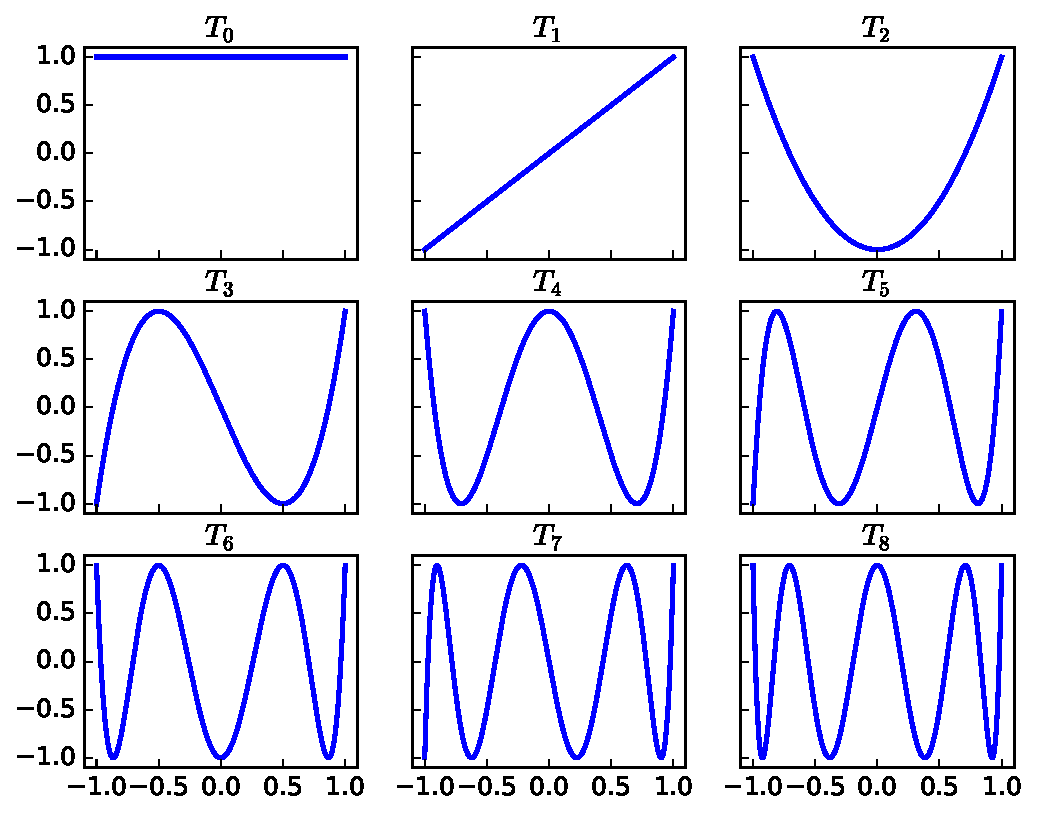
\includegraphics[width=.7\linewidth]{figures/chebyshev_good.pdf}
\end{figure}

\begin{info} % LaTex with Matplotlib text.
Matplotlib titles and annotations can be formatted with \LaTeX, a system designed for creating technical and scientific documents%
\footnote{See \url{http://www.latex-project.org/} for more information.}
(this lab manual, for example, is written in \LaTeX).
To do so, use an `r' before the string quotation mark) and surround the text with dollar signs.

For example, try replacing the final line of code in the previous example with the following line.

\begin{lstlisting}
...     plt.title(r"$T_{}(x)$".<<format>>(n))
\end{lstlisting}

The string's \li{<<format>>()} method inserts the input $n$ at the curly braces.
The title of the sixth subplot, instead of being ``n = 5,'' will then be ``$T_5$.''
\end{info}

% TODO: Make sure the Bernstein polynomial notation is consistent with the book (it is consistent with Wikipedia currently)

\begin{problem} % Plot the Bernstein polynomials.
The $n+1$ Bernstein basis polynomials of degree $n$ are defined as follows.
\[b_{v,n} = {{n} \choose {v}} x^v (1-x)^{n-v},\qquad v = 0,\ 1,\ \ldots,\ n\]

Plot at least the first $10$ Bernstein basis polynomials ($n = 0,\ 1,\ 2,\ 3$) as small multiples on the domain $[0,1] \times [0,1]$.
Label the subplots for clarity, adjust tick marks and labels for simplicity, and set the window limits of each plot to be the same.
Consider arranging the subplots so that the rows correspond with $n$ and the columns with $v$.
\\(Hint: The constant ${{n} \choose {v}} = \frac{n!}{v!(n-v)!}$ is called the \emph{binomial coefficient} and can be efficiently computed with \li{scipy.special.binom()} or \li{scipy.misc.comb()}.)
\end{problem}

\subsection*{Scatter Plots} % -------------------------------------------------

A scatter plot draws $(x,y)$ points without connecting them.
Connecting the points would imply an order or relation between the points, so scatter plots are best for displaying data sets without a natural order, or where each point is a distinct, individual instance.

Consider the following questions when making a scatter plot.
Note that some of them are the same questions that should be asked when creating a line plot.
%
\begin{itemize}
    \item What do the axes represent? How should they be labeled?
    \item Would a linear scale or a logarithmic scale most clearly reveal patterns?
    \item What should the window limits be?
    \item Which marker is best? Are the markers an appropriate size and color?
\end{itemize}

A scatter plot can be drawn with either \li{plt.plot()} (specify a point marker such as \li{'.'}, \li{','}, \li{'o'}, or \li{'+'}) or \li{plt.scatter()}.
While \li{plt.plot()} is the more flexible function in general, \li{plt.scatter()} provides a few extra tools.
Most useful are the keywords \li{s} and \li{c}, which correspond to marker size and marker color, respectively.
Each keyword can either be a single entry or an array.
Using an array specifies the sizes or colors of each individual marker, allowing a scatter plot to have up to four dimensions of information.

\begin{comment}
% Window size, also should go later.
Figure \ref{fig:scatter_correlation} displays two scatter plots.
The first appears to have a weak correlation and the second appears to have a strong correlation.
However, the same data is being plotted and the only difference is the scale and window size.
Manipulating these can change your interpretation and should be done with careful consideration.
\end{comment}

Consider a collection of rectangular boxes where the lengths, widths, and heights are given.
A scatter plot of length against width mostly describes the sizes of the boxes; tying the third dimension (height) to the color of the points can provide the additional information.
Setting the marker size of the marker as the volume of the boxes also adds some depth to the visualization, though modifying both the color and the size might be considered overkill.

Since adjusting the marker size may lead to overlapping points, we specify the \emph{alpha value} of the color to make the markers slightly transparent.
The keyword \li{alpha} accepts a value in the interval $[0,1]$; 0 makes the markers completely transparent, while a $1$ makes the markers completely opaque.

Finally, as with heat maps and contour plots, a color bar can be added with \li{plt.colorbar()} to indicate the values that the colors represent.
This color bar can be given a label as well.

\begin{lstlisting}
>>> length, width, height = np.random.randint(1, 20, (3,50))

>>> plt.subplot(221)                # Plot length against width.
>>> plt.scatter(length, width, s=100)
>>> plt.grid()
>>> plt.ylabel("Width (inches)")
>>> plt.tick_params(labelbottom="off")
>>> plt.axis([0, 20, 0, 20])

>>> plt.subplot(222)                # Set the marker color to the height.
>>> plt.scatter(length, width, c=height, s=100)
>>> cbar = plt.colorbar()
>>> cbar.set_label("Height (inches)")
>>> plt.grid()
>>> plt.tick_params(labelbottom="off", labelleft="off")
>>> plt.axis([0, 20, 0, 20])

>>> plt.subplot(223)                # Set the marker size to half the volume.
>>> plt.scatter(length, width, s=length*width*height/2., alpha=.7)
>>> plt.grid()
>>> plt.xlabel("Length (inches)")
>>> plt.ylabel("Width (inches)")
>>> plt.axis([0, 20, 0, 20])

>>> plt.subplot(224)                # Use color and marker size together.
>>> plt.scatter(length, width, c=height, s=length*width*height/2., alpha=.7)
>>> cbar = plt.colorbar()
>>> cbar.set_label("Height (inches)")
>>> plt.grid()
>>> plt.tick_params(labelleft="off")
>>> plt.xlabel("Length (inches)")
>>> plt.axis([0, 20, 0, 20])
\end{lstlisting}

\begin{figure}[H] % Scatter plots.
\captionsetup[subfigure]{justification=centering}
\centering
\begin{subfigure}{.495\textwidth}
    \centering
    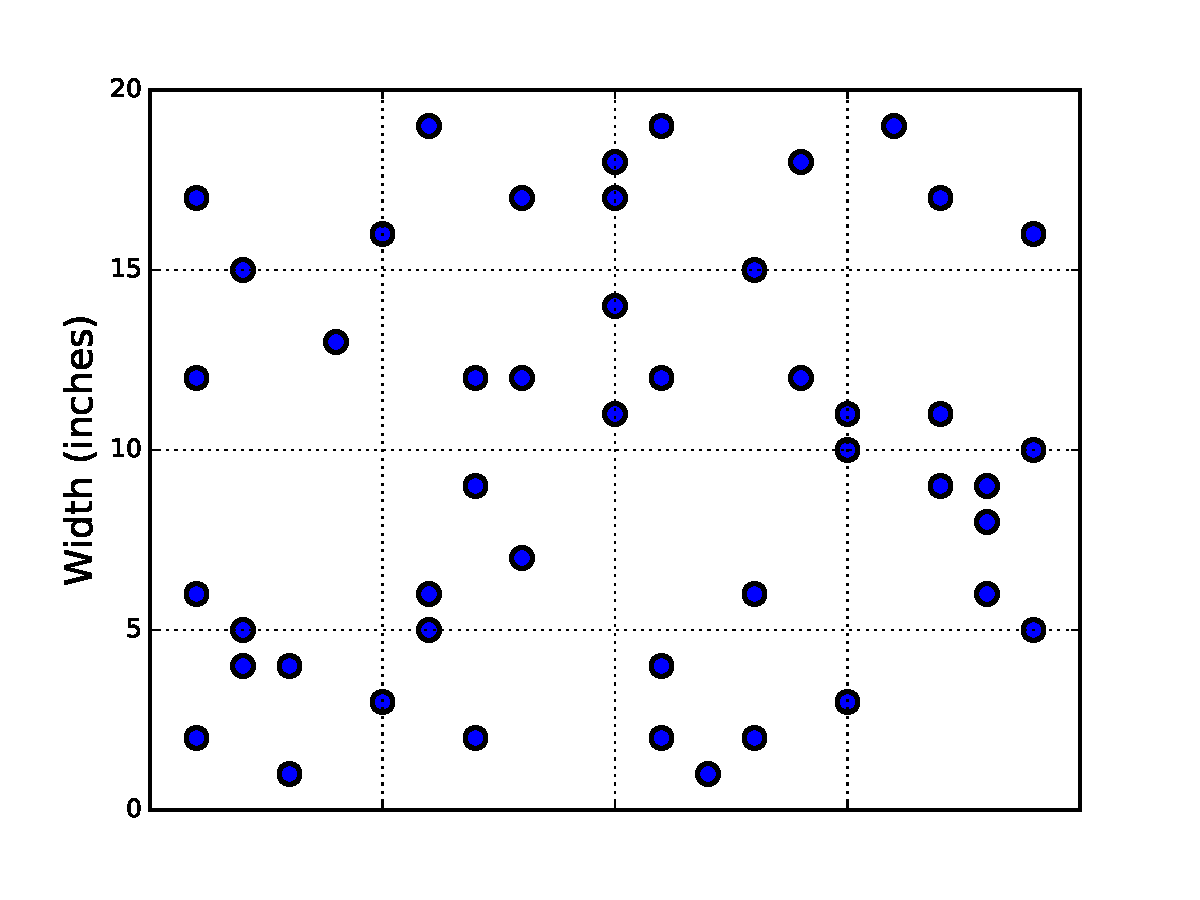
\includegraphics[width=\linewidth]{figures/scatter_1.pdf}
\end{subfigure}
%
\begin{subfigure}{.495\textwidth}
    \centering
    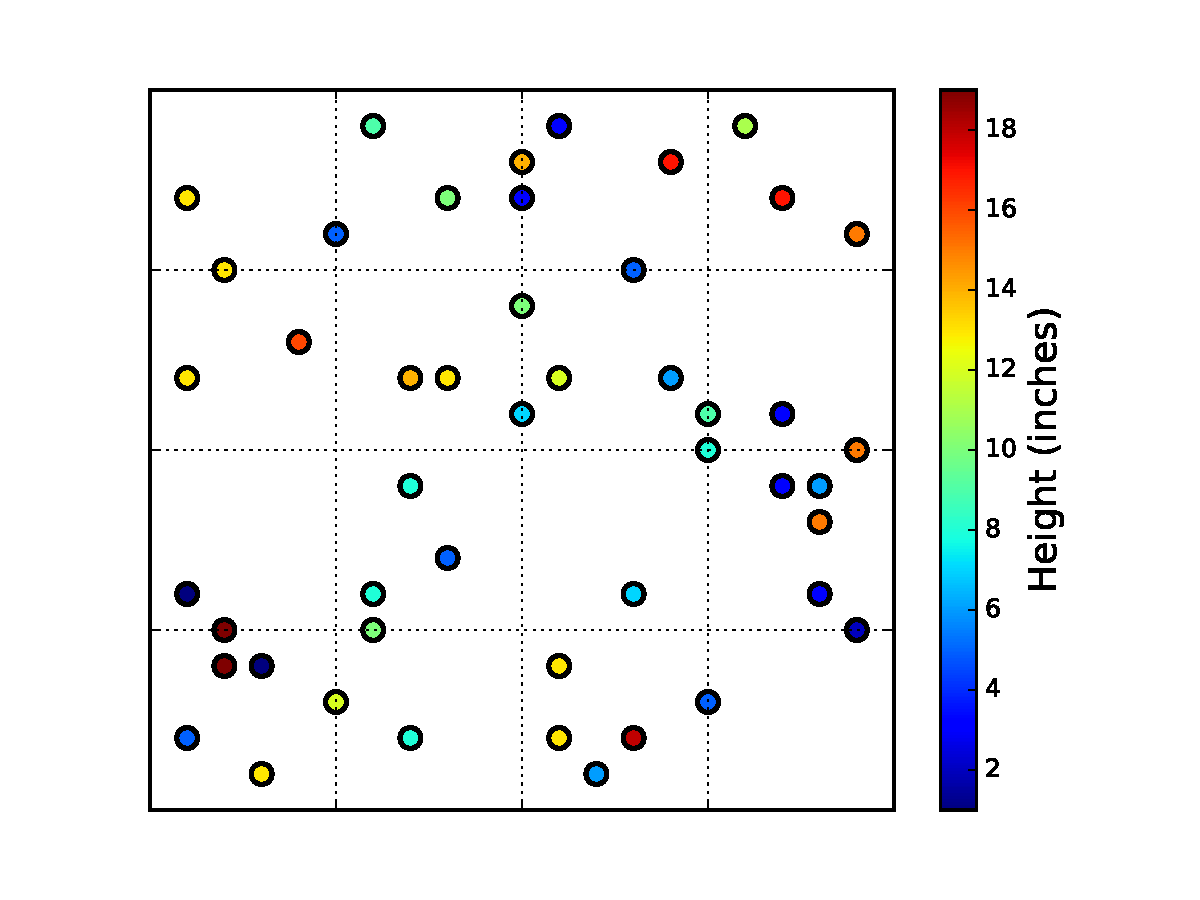
\includegraphics[width=\linewidth]{figures/scatter_2.pdf}
\end{subfigure}
\\
\begin{subfigure}{.495\textwidth}
    \centering
    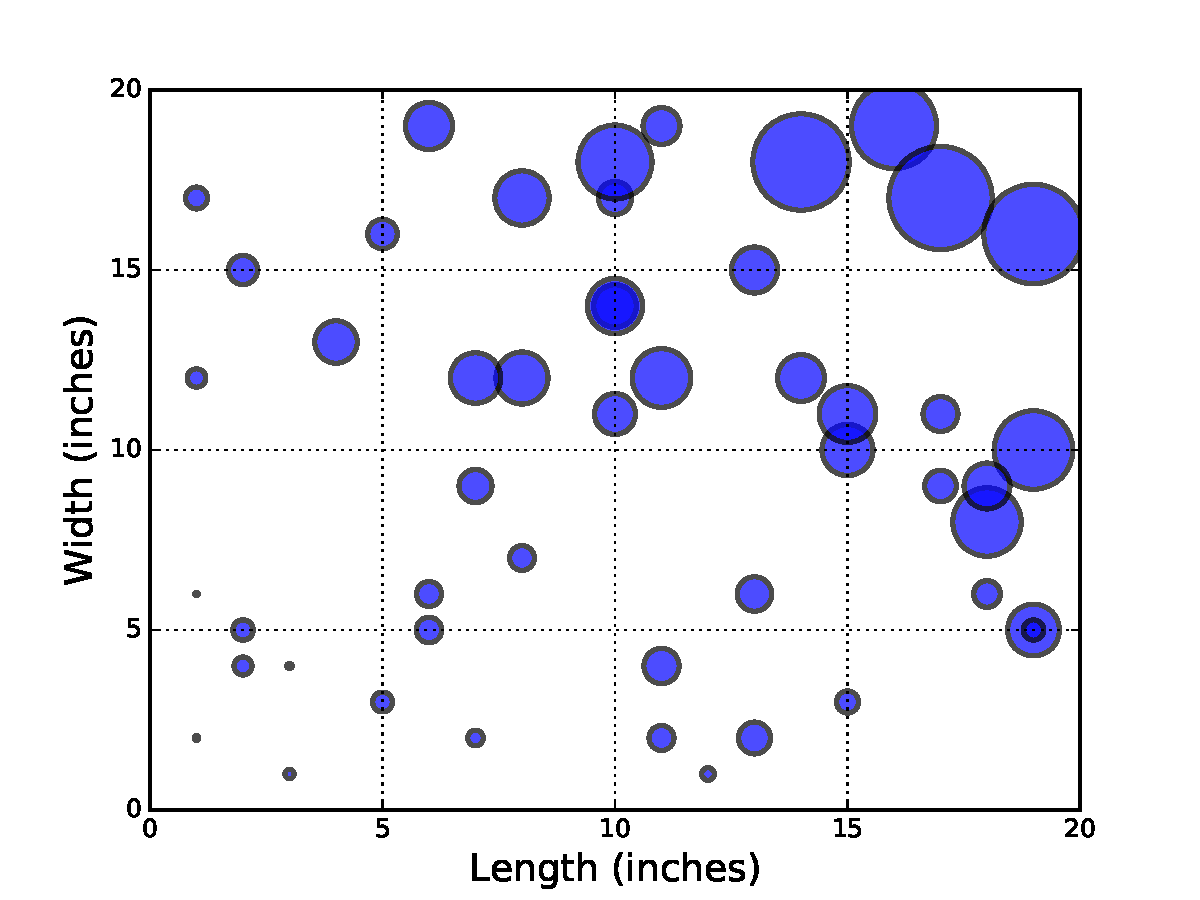
\includegraphics[width=\linewidth]{figures/scatter_3.pdf}
\end{subfigure}
%
\begin{subfigure}{.495\textwidth}
    \centering
    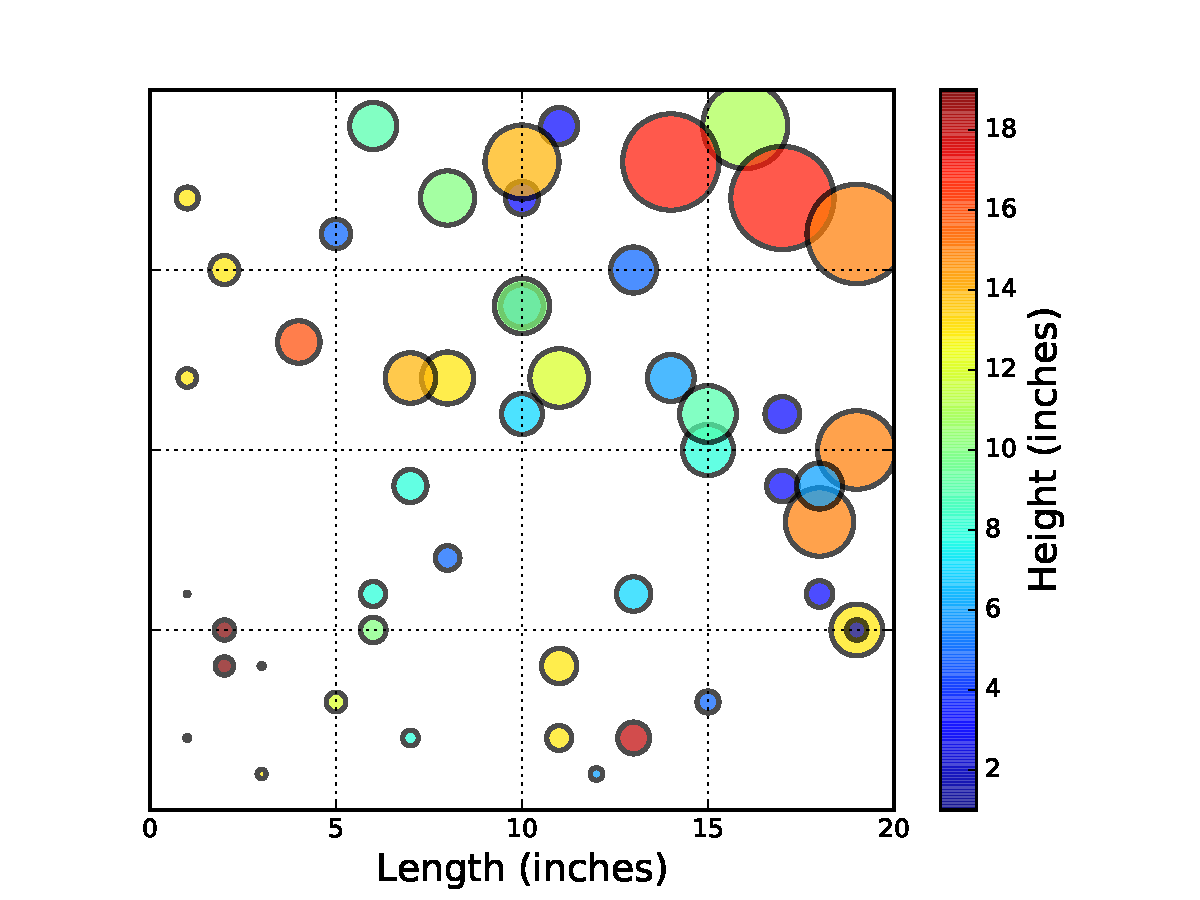
\includegraphics[width=\linewidth]{figures/scatter_4.pdf}
\end{subfigure}
\end{figure}

In scatter plots, connecting the points into a line plot usual results in extreme clutter.
A regression line, however, highlights a pattern in the data without overshadowing the actual data points.%
\footnote{See the Least Squares lab (QR 2), especially Problems 2–--4, for a refresher on regression lines.}

\begin{problem} % Scatter plots with visualizations.
The file \texttt{MLB.npy} contains measurements from over 1,000 recent Major League Baseball players, compiled by UCLA.\footnote{See \url{http://wiki.stat.ucla.edu/socr/index.php/SOCR_Data_MLB_HeightsWeights}.}
Each row in the array represents a different player; the columns are the player's height (in inches), weight (in pounds), and age (in years), in that order.

Describe the data with at least one scatter plot.
Your graph(s) should demonstrate whether height, weight, or age correlated with each other in the MLB.
Consider plotting the linear regression line to indicate trends.
\end{problem}

% DONE TO HERE = = = = = = = = = = = = = = = = = = = = = = = = = = = = = = = =

\subsection*{Histograms} % ----------------------------------------------------

\begin{comment}

\textbf{Histogram}: Partitions an interval into a number of bins and counts the number of values that fall into each bin.

Best for visualizing a single unordered array, such as draws from a probability distribution.
%
\begin{itemize}
    \item How many bins should be used?
    \item Over what range should the bins be?
    \item Is a linear or a logarithmic scale more appropriate for the frequency axis?
\end{itemize}

% Use \li{plt.hist()} to create a histogram.
% The arguments \li{bins} and \li{<<range>>} specify the number of bins to draw and over what domain.

% Details for later.
A histogram with only a few bins or too many bins will fail to give a clear view of the distribution of the data, therefore it is important to choose the number of bins that gives the best view of the distribution of the data.

Similarly, reference lines are distracting and focus on unnecessary details instead of the shape of the distribution.
If more precise details are desired, exact figures can be presented alongside the histogram in a table.

\textbf{Heat Map}: Assigns a color to each point on a 2-D domain, providing a 2-D picture representing a 3-D surface.

Best for visualizing functions $f:\mathbb{R}^2\rightarrow\mathbb{R}$, usually over a domain constructed with \li{np.meshgrid()}.
%
\begin{itemize}
    \item Is the domain sufficiently refined?
    \item Which color scheme is most clear and effective?
    \item Is a linear or a logarithmic scale more appropriate for the color?
\end{itemize}

\textbf{Contour Map}: Draws level curves of a function $f:\mathbb{R}^2\rightarrow\mathbb{R}$.

A filled contour map is discretized version of a heat map.
%
\begin{itemize}
    \item How many / which contour lines should be drawn?
    % \item Is the color scheme clear and effective?
    \item Is a linear or a logarithmic scale more appropriate for the color?
\end{itemize}

\end{comment}
%
% \begin{table}[H]
% \begin{tabular}{rcc}
% & \textbf{One Array} & \textbf{Two Arrays} \\
% \cline{2-3}
% \textbf{Ordered Data} &
% \multicolumn{1}{|c|}{Line Plot} & \multicolumn{1}{|c|}{Line Plot} \\
% \cline{2-3}
% \textbf{Unordered Data} &
% \multicolumn{1}{|c|}{Histogram} & \multicolumn{1}{|c|}{Scatter Plot} \\
% \cline{2-3}
% % \textbf{Categorical Data} & \multicolumn{1}{|c|}{Bar Chart} & \multicolumn{1}{|c|}{Scatter Plot} \\ \cline{2-3}
% \end{tabular}
% \end{table}


Line plots should \emph{not} be used for data without a natural progression.
For example, suppose we would like to make a large number of random draws from a distribution to visualize its probability density function.
In this case, a plain line plot is completely useless, but the histogram provides an accurate picture of the statistical distribution.

\begin{comment}
\begin{lstlisting}
>>> import numpy as np
>>> from matplotlib import pyplot as plt

# Get 10,000 random samples from the standard normal distribution.
>>> data = np.random.normal(size=10000)

>>> plt.subplot(121)                # Regular line plot of the data.
>>> plt.plot(data)

>>> plt.subplot(122)                # Histogram of the data.
>>> plt.hist(data, bins=30)

>>> plt.show()
\end{lstlisting}

\begin{figure}[H] % line plot versus a histogram.
\captionsetup[subfigure]{justification=centering}
\centering
\begin{subfigure}{.49\textwidth}
    \centering
    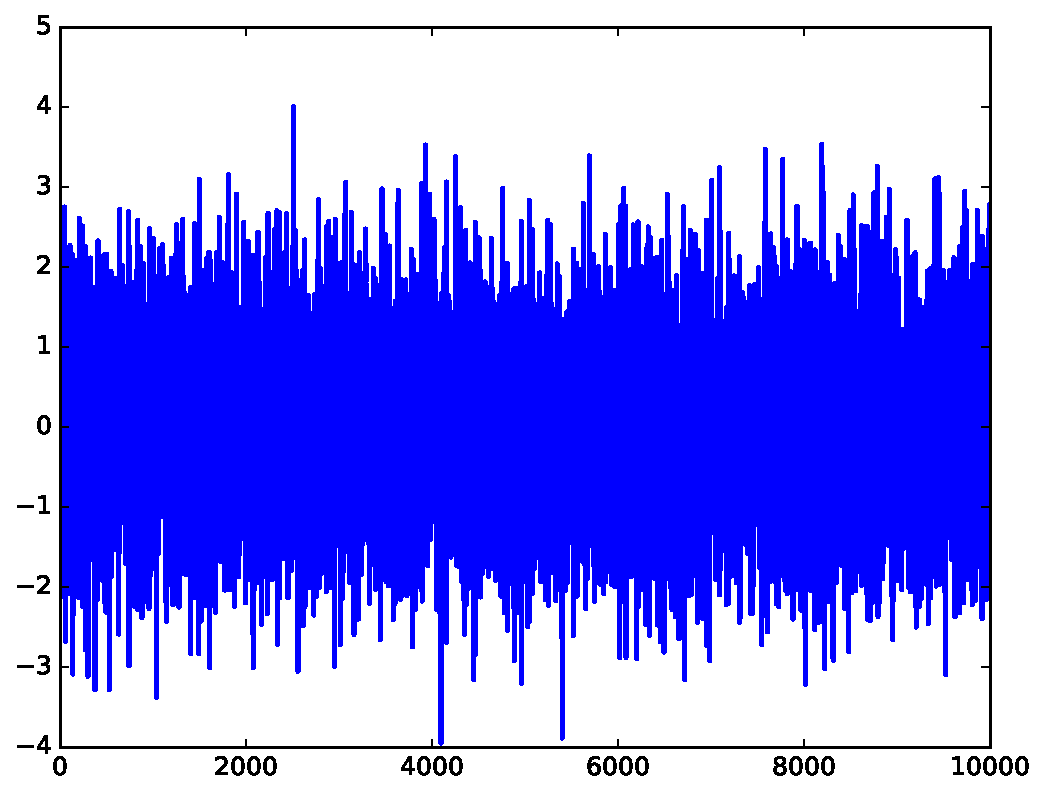
\includegraphics[width=\linewidth]{figures/hist_1_bad.pdf}
\end{subfigure}
%
\begin{subfigure}{.49\textwidth}
    \centering
    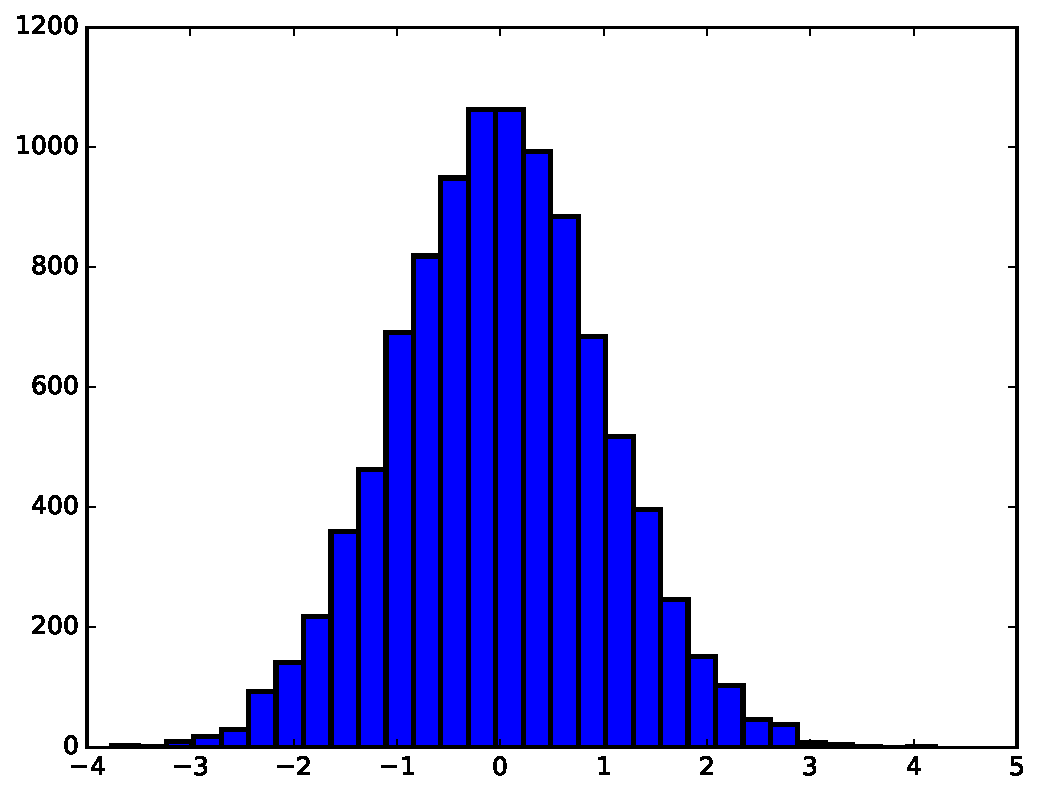
\includegraphics[width=\linewidth]{figures/hist_1_good.pdf}
\end{subfigure}
\end{figure}
\end{comment}

Less is more.
In the case of a statistical distribution, all we really want to see is the general shape of the distribution.
The lines separating the bins, axis tick marks, and even the labels on the $y$ axis are all unnecessary (and potentially distracting) details.

Removing the lines between bins is easy: set the line width to $0$.
To ensure the gaps where the lines used to be are filled, specify the \li{histtype} as \li{"stepfilled"} (using \li{histtype="step"} will draw the outline without filling it in).
Finally, to get rid of extra markings on the axes, use \li{plt.tick_params()}.

\begin{lstlisting}
# Get 10,000 random samples from the standard exponential distribution.
>>> data = np.random.exponential(size=N)

>>> plt.subplot(121)
>>> plt.hist(data, bins=30)

>>> plt.subplot(122)                # Histogram with no lines or tick marks.
>>> plt.hist(data, bins=30, lw=0, histtype="stepfilled")
>>> plt.tick_params(axis="both", which="both", labelleft='off',
...                              left="off", top="off", right="off")

>>> plt.show()
\end{lstlisting}

\begin{figure}[H] % Cleaning up a histogram.
\captionsetup[subfigure]{justification=centering}
\centering
\begin{subfigure}{.49\textwidth}
    \centering
    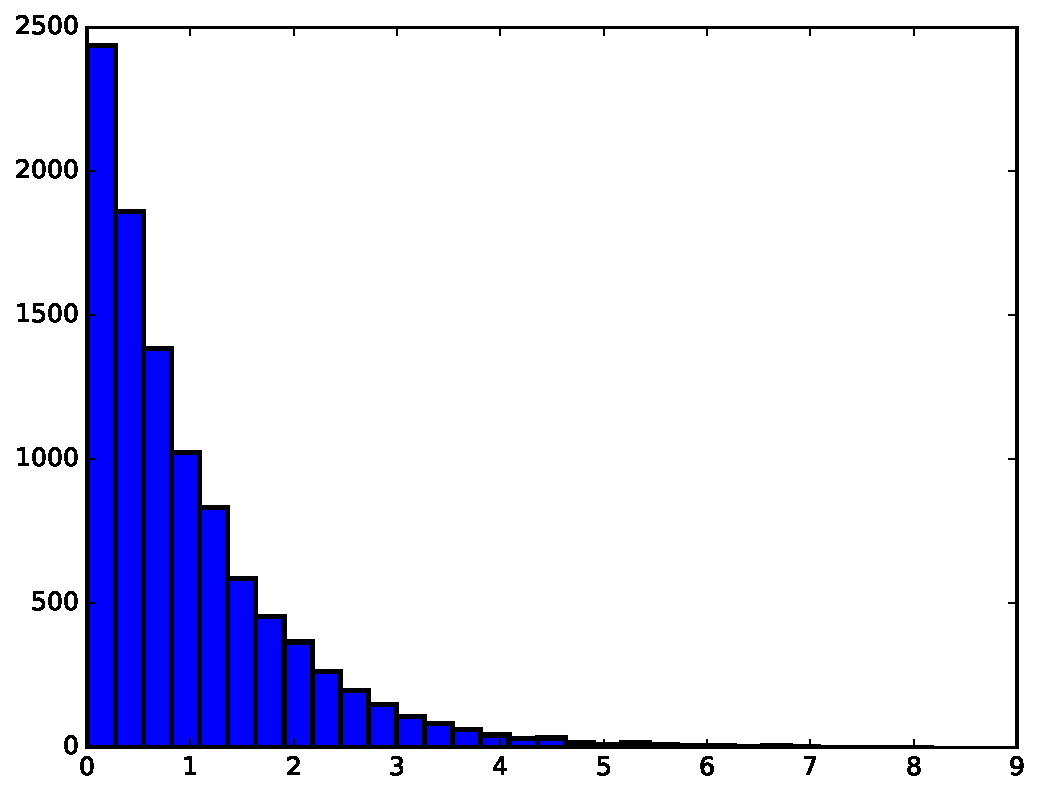
\includegraphics[width=\linewidth]{figures/hist_2_bad.pdf}
\end{subfigure}
%
\begin{subfigure}{.49\textwidth}
    \centering
    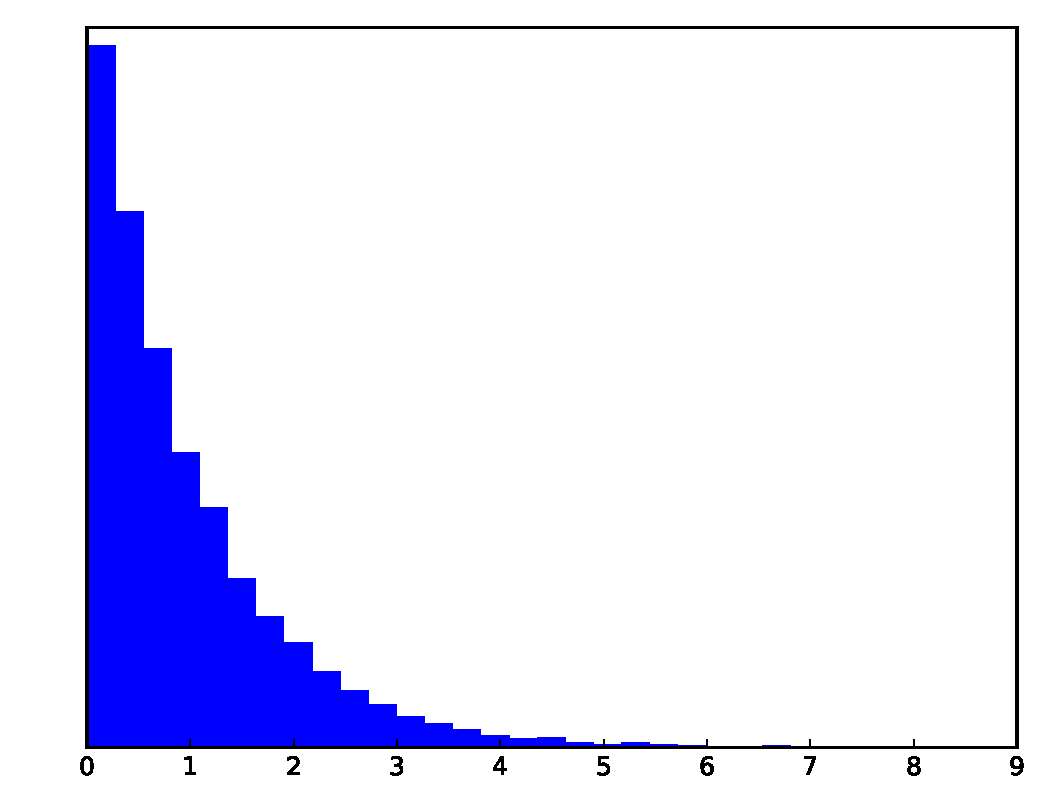
\includegraphics[width=\linewidth]{figures/hist_2_good.pdf}
\end{subfigure}
\end{figure}

A histogram plots an array of values against the frequency with which the values occur.
To plot a line plot of values against frequency (without drawing a histogram), use \li{np.histogram()}.
This function returns the number of values in each bin and the locations of the edges of the bins.
Use the edges of the bins to calculate the center of the bins, then use a line plot to connect the two.

\begin{lstlisting}
# Get samples from a beta distribution and draw its PDF.
>>> for i, N in enumerate([10000, 10000000]):
...     plt.subplot(1,2,i+1)
...     data = np.random.beta(a=5, b=2, size=N)
...     # Draw a line plot using the bin centers and frequencies.
...     frequencies, bin_edges = np.histogram(data, bins=50)
...     bin_centers = (bin_edges[:-1] + bin_edges[1:])/2.
...     plt.plot(bin_centers, frequencies, 'b-', lw=4)
...     # Plot the faded histogram for comparison.
...     plt.hist(data, bins=50, alpha=.1)
...     plt.tick_params(axis="both", which="both", labelleft='off',
...                                  left="off", top="off", right="off")
...
>>> plt.show()
\end{lstlisting}

\begin{figure}[H] % Histogram Line Plot Hybrid
\captionsetup[subfigure]{justification=centering}
\centering
\begin{subfigure}{.49\textwidth}
    \centering
    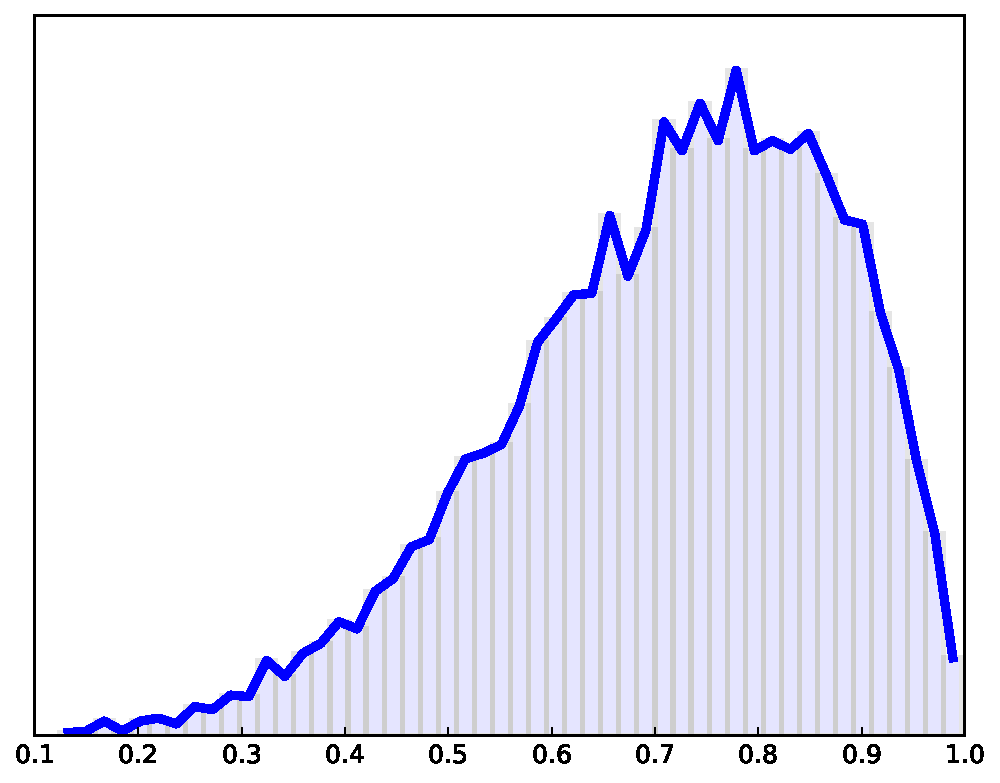
\includegraphics[width=\linewidth]{figures/hist_3_bad.pdf}
\end{subfigure}
%
\begin{subfigure}{.49\textwidth}
    \centering
    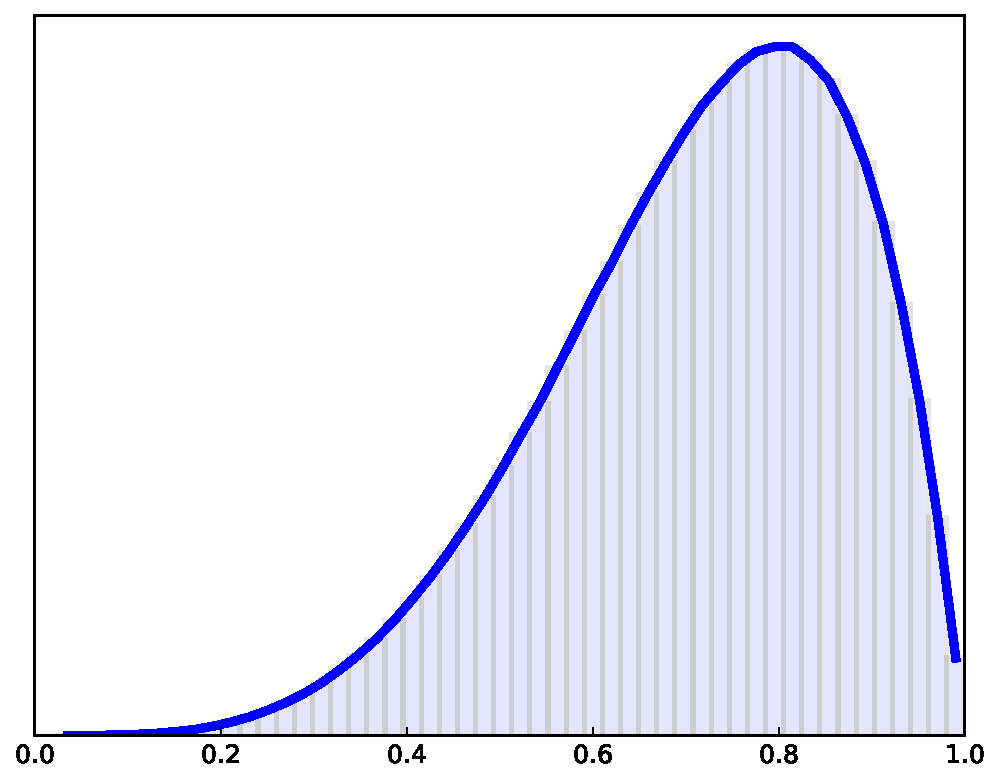
\includegraphics[width=\linewidth]{figures/hist_3_good.pdf}
\end{subfigure}
\end{figure}

\begin{problem} % Earthquake data
The file \texttt{earthquakes.npy} contains data from the 17,065 earthquakes between 2000 and 2010 that were at least a 5 on the Richter scale.\footnote{See \url{http://earthquake.usgs.gov/earthquakes/search/}.}
Each row in the array represents a different earthquake;
the columns are the earthquake's date (as a fraction of the year), magnitude, longitude, and latitude, in that order.

Because each earthquake is a distinct event, a good way to start visualizing this data might be a scatter plot of the years versus the magnitudes of each earthquake.

\begin{lstlisting}
>>> year, magnitude, longitude, latitude = np.load("earthquakes.npy").T
>>> plt.plot(year, magnitude, '.')
>>> plt.xlabel("Year")
>>> plt.ylabel("Magnitude")
>>> plt.show()
\end{lstlisting}

\begin{figure}[H] % Bad visualization: earthquake data, year vs magnitude.
    \centering
    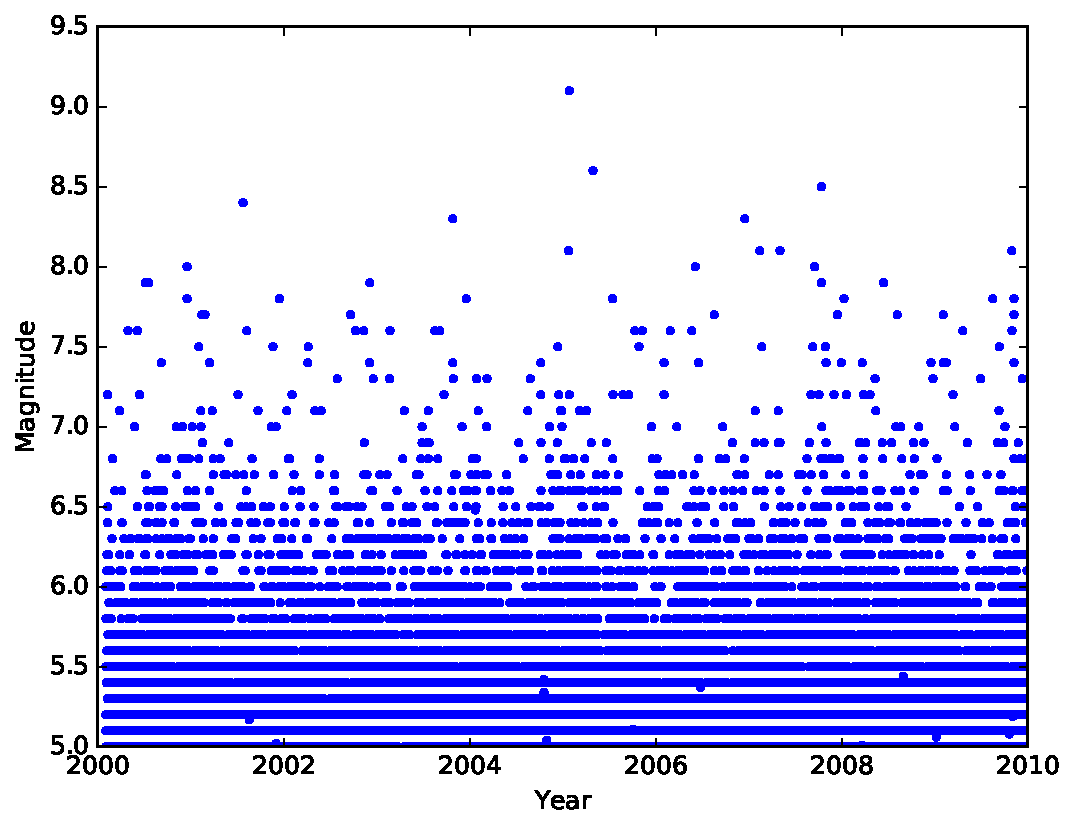
\includegraphics[width=.7\textwidth]{figures/earthquake.pdf}
\end{figure}

Unfortunately, this plot communicates very little information because the data is so cluttered.
Describe the data with two or three better visualizations.
Your graphs should clearly answer the following questions:
\begin{enumerate}
    \item How many earthquakes happened every year?
    \item How often do stronger earthquakes happen compared to weaker ones?
    \item Where do earthquakes happen? Where do the strongest earthquakes happen?
\end{enumerate}
% (Hint: \li{plt.gca().set_aspect("equal")} fixes the aspect ratio, which may improve comparisons between longitude and latitude.)
\end{problem}

% Consider Figure \ref{fig:logexample} which shows data about large earthquakes from the United States Geological Survey.
% It appears to be somewhat random however, when transformed, the frequency of the magnitudes on a logarithmic scale show a fairly strong linear relationship between the variables.

\subsection*{Heat and Contour Maps} % -----------------------------------------

\begin{figure}[h]
\centering
\begin{subfigure}{.45\textwidth}
\centering
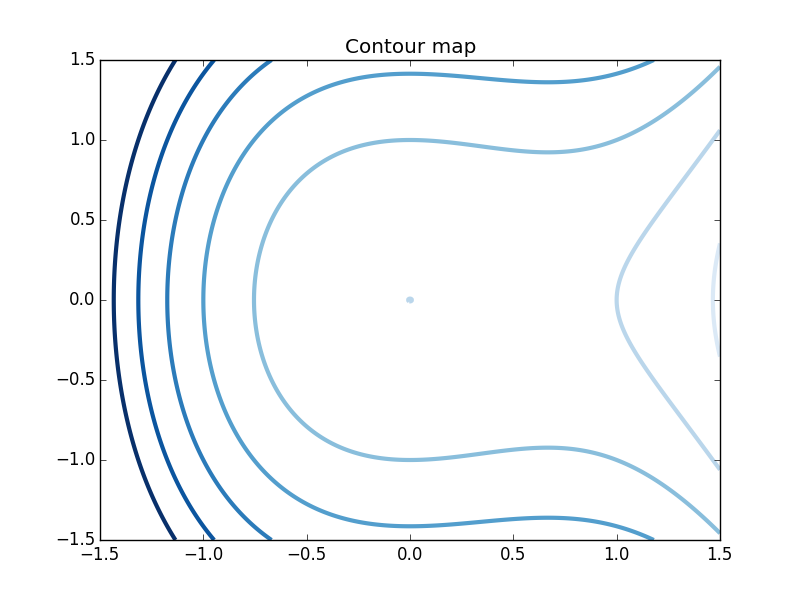
\includegraphics[width=\textwidth]{contour_map.png}
\end{subfigure}
\begin{subfigure}{.45\textwidth}
\centering
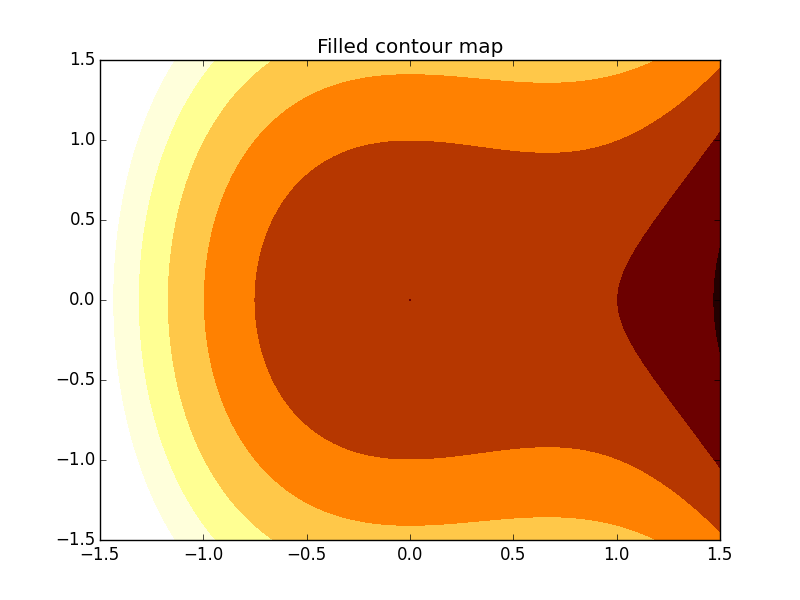
\includegraphics[width=\textwidth]{contour_map_filled.png}
\end{subfigure}
\begin{subfigure}{.45\textwidth}
\centering
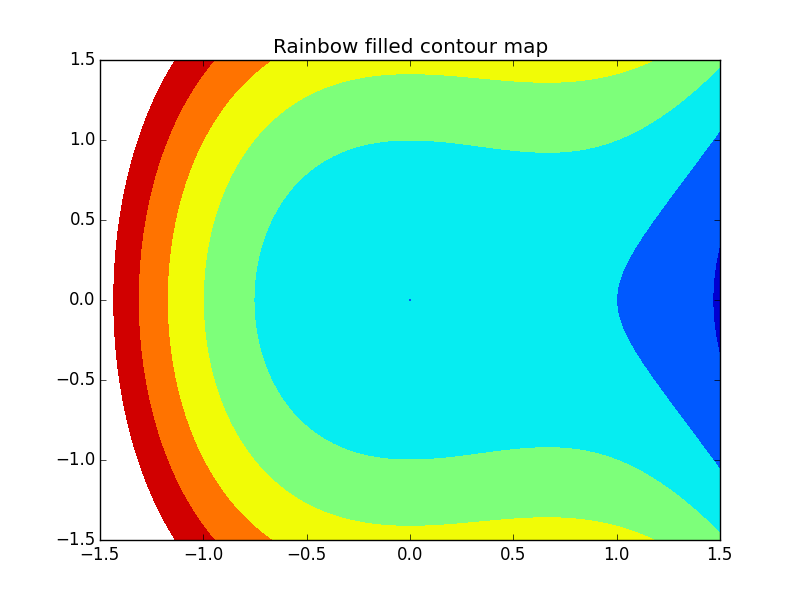
\includegraphics[width=\textwidth]{contour_map_rainbow_filled.png}
\end{subfigure}
\begin{subfigure}{.45\textwidth}
\centering
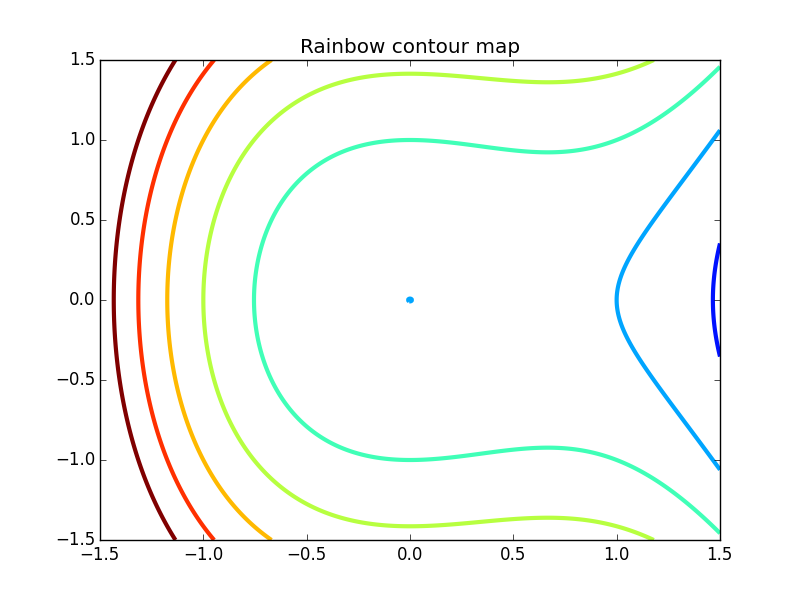
\includegraphics[width=\textwidth]{contour_map_rainbow.png}
\end{subfigure}
\caption{Contour Maps.  A contour map (top left) and a heat map (top right).
The color choices of the bottom row are less intuitive and make the visualization harder to interpret.}
\label{fig:contour}
\end{figure}

Three-dimensional data can be displayed with a contour plot.
This draws lines in the plane where the third value is constant---like a topographical map.
Coloring the space between the contour lines produces a heat map.
Heat maps work best when only one or two colors are used.

\begin{figure}[h]
\centering
\begin{subfigure}{.5\textwidth}
  \centering
  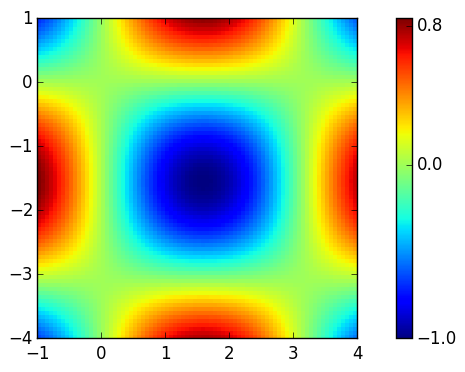
\includegraphics[width=\textwidth]{heatmap_color.png}
\end{subfigure}%
\begin{subfigure}{.5\textwidth}
  \centering
  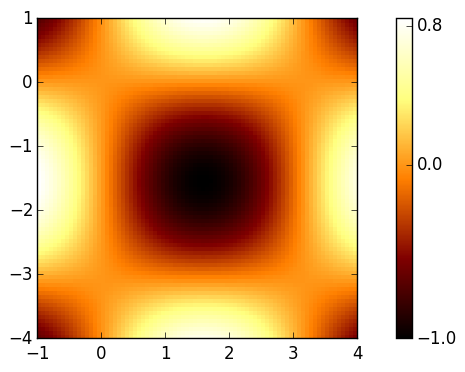
\includegraphics[width=\textwidth]{heatmap_hot.png}
\end{subfigure}
%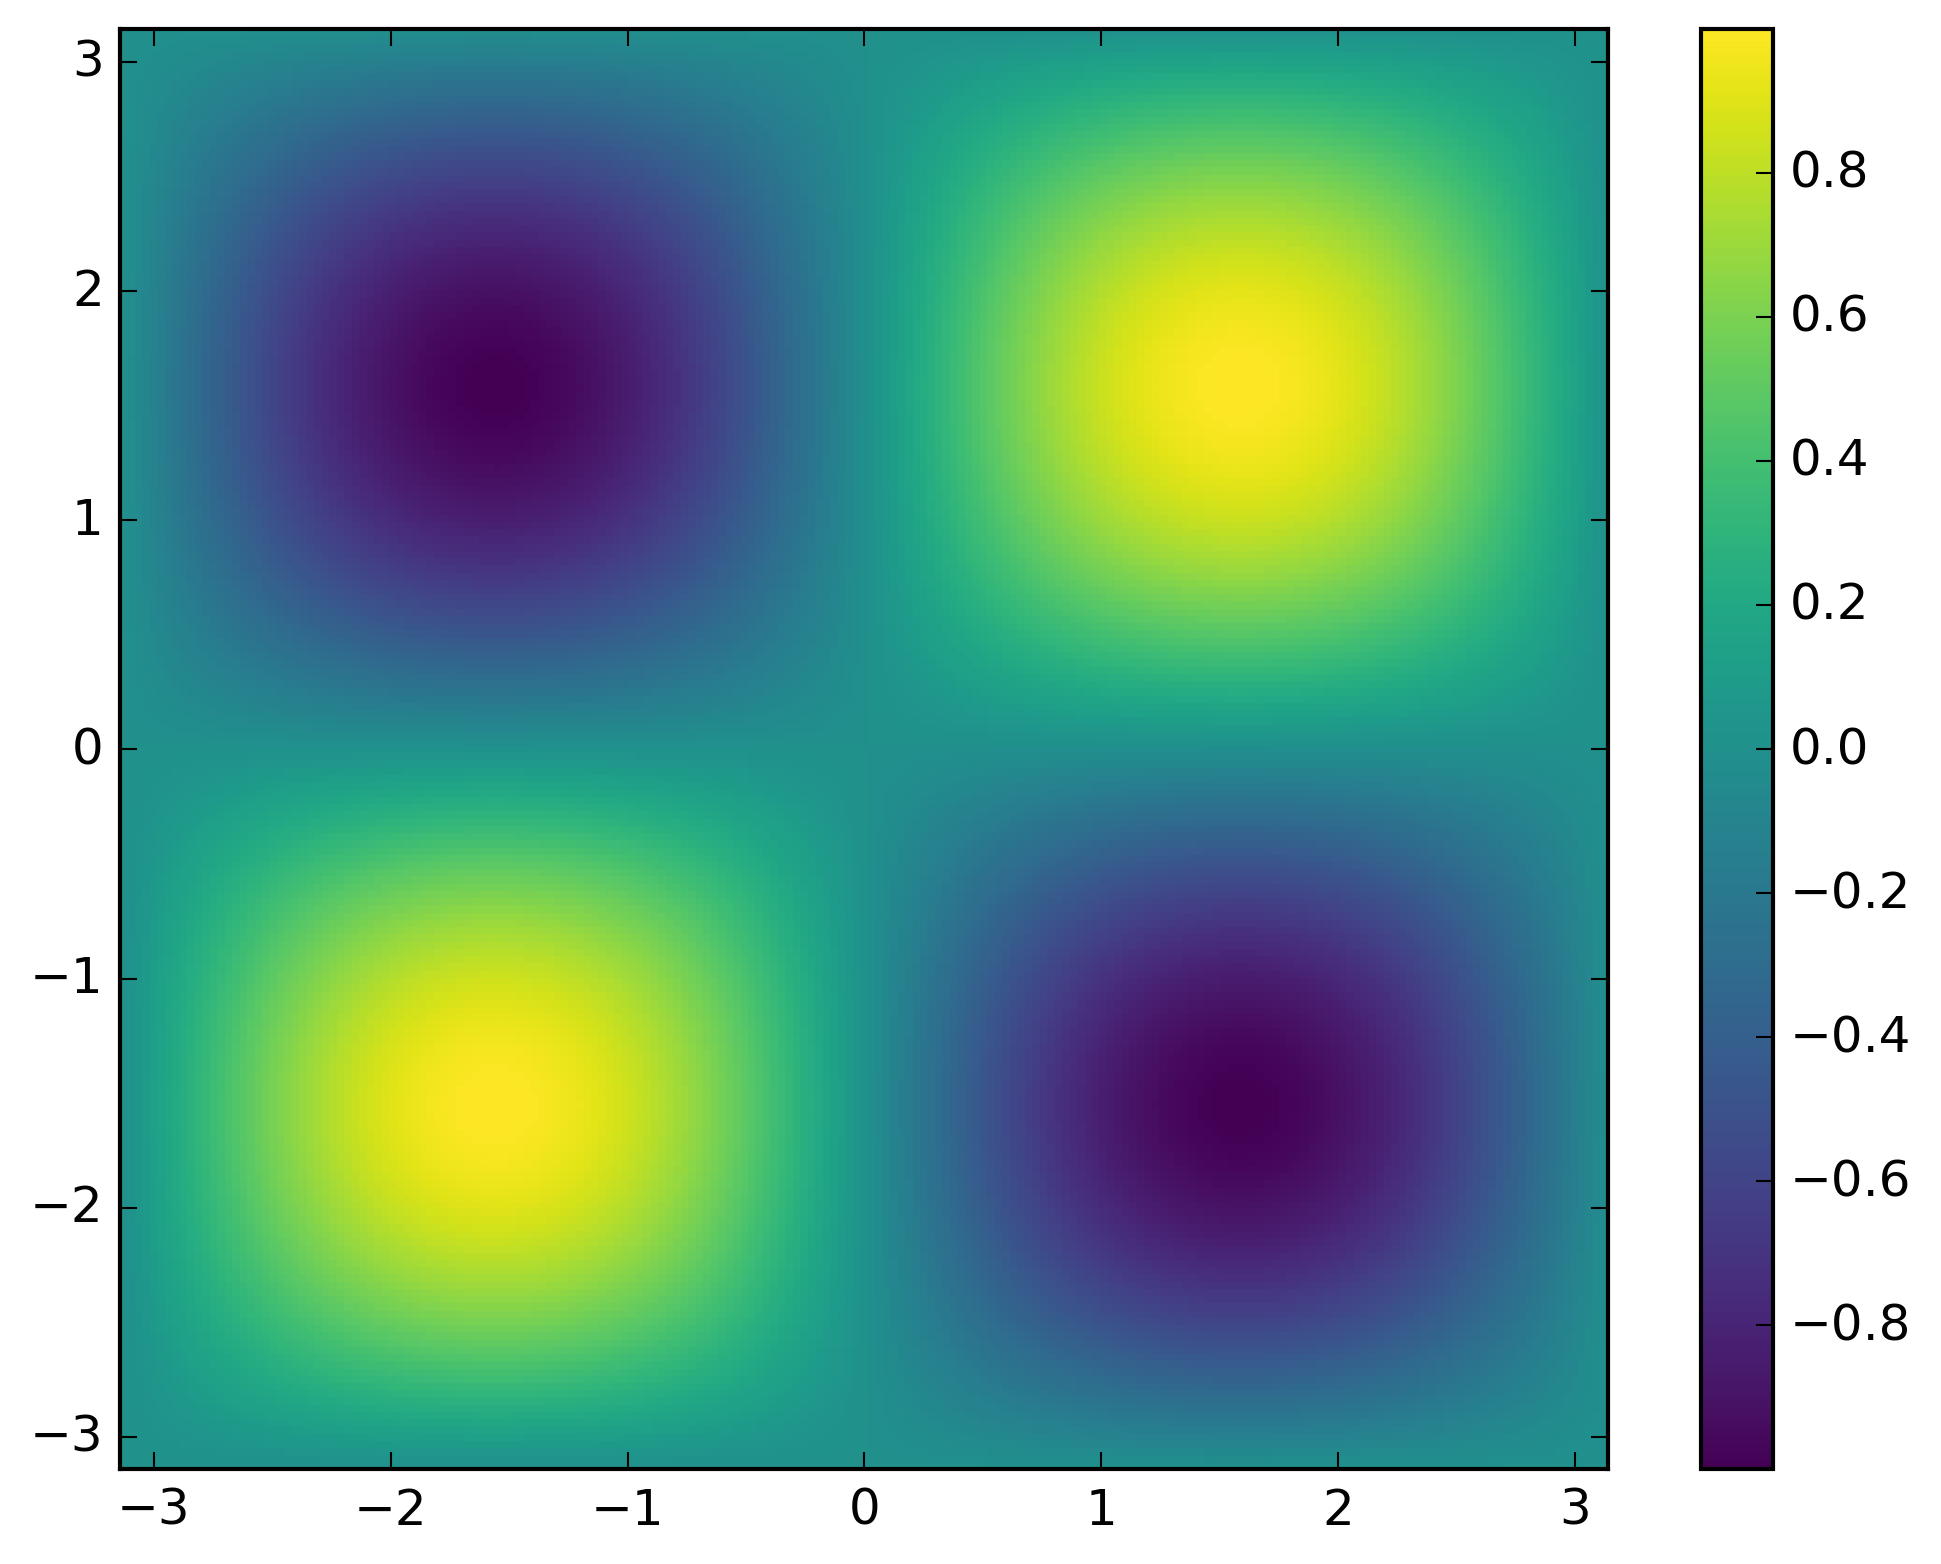
\includegraphics[width=\textwidth]{heatmap.png}
\caption{Both of these pseudocolor plots depict the function
    $z = \sin(x)\sin(y)$ on the domain $[-1,4] \times [-4,1]$.
The plot on the left uses a rainbow gradient, which has no meaningful relationship to the data.
The plot on the right uses the colormap \li{afmhot}.  The lighter and darker colors are a more intuitive
representation of higher and lower values.}

\label{fig:heatmap}
\end{figure}

% TODO: In the next release of Matplotlib (version 2.0) viridis is the default.
% TODO: Reword (awkward).
A good default colormap is Matplotlib's \li{viridis}.
Other colormaps that are appropriate for the data can be selected using the argument \li{cmap='NAME\_OF\_COLORMAP'}, where \li{NAME\_OF\_COLORMAP} is one of Matplotlib's sequential or diverging colormaps.
Two sequential colormaps are \li{afmhot} and \li{cool}. Two diverging colormaps are \li{seismic} and \li{bwr}.
These colormaps along with their color scheme can be found on
\url{http://matplotlib.org/examples/color/colormaps_reference.html}.
Although three-dimensional data can be plotted as a surface in 3-space, it is often difficult to find a view where none of the important features of the data are obscured.
A heatmap avoids this problem and is easier to understand.

You can create a contour plot in Matplotlib with \li{plt.contour()}.

You can also create a pseudocolor plot in Matplotlib with the \li{plt.pcolormesh()} command.

% # This code corresponds to the figure on the top right of the contour maps.
\begin{lstlisting}
import numpy as np
from matplotlib import pyplot as plt

n=400
xran = np.linspace(-1.5,1.5,n)
yran = np.linspace(-1.5,1.5,n)
X, Y = np.meshgrid(xran,yran)
F = Y**2 - X**3 + X**2
plt.contourf(X, Y, F, [-2,-1,0.0001,1,2,3,4,5] ,cmap=plt.get_cmap('afmhot'))
\end{lstlisting}

\begin{problem} % Contour map problem. TODO: don't specify number of intervals?
Using 400 intervals, plot a filled contour map of the function \[f(x,y) = \sin(x) + \sin(y)\] over the domain $[0,12\pi]\times[0,12\pi]$.

Be sure to use an appropriate color map.
\end{problem}

\section*{Communicating Insights with Visualizations} % =======================

\begin{comment} % USE THIS AS AN EXAMPLE LATER.
\begin{figure}[H] % Histogram with and without busy information.
\centering
\begin{subfigure}{.45\textwidth}
\centering
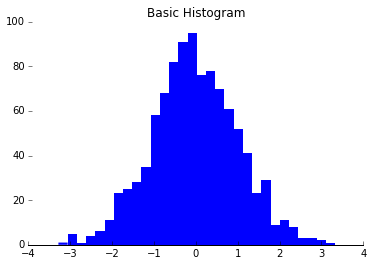
\includegraphics[width=\textwidth]{good_hist_example.png}
\end{subfigure}
\centering
\begin{subfigure}{.45\textwidth}
\centering
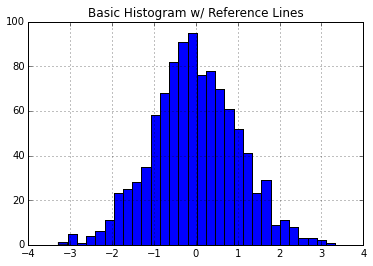
\includegraphics[width=\textwidth]{hist_reference_grid.png}
\end{subfigure}
\caption{Histogram with and without reference lines. It is harder to see the shape of the distribution in the histogram with reference lines.}
\label{fig:histogram}
\end{figure}

Plot two histograms with data drawn randomly from a normal and exponential distribution.

\begin{lstlisting}
from numpy.random import normal
from numpy.random import exponential
normal_data = normal(size=1000)
exp_data = exponential(size=1000)
\end{lstlisting}

For each distribution, plot a histogram using 30 bins, 15 bins and 5 bins.
Does this change how we interpret the distribution of the data?
\end{comment}

\begin{comment}
\begin{figure}[h] % Line plots.
\centering
\begin{subfigure}{.45\textwidth}
\centering
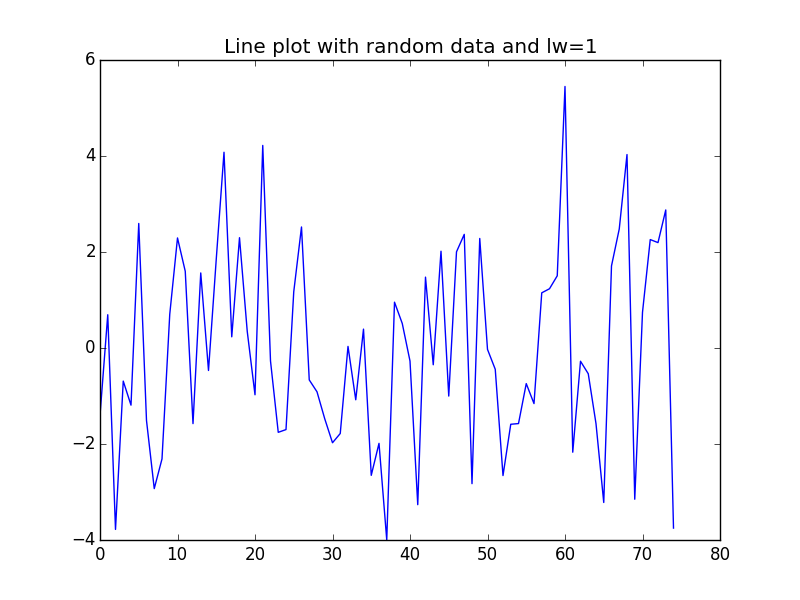
\includegraphics[width=\textwidth]{line_plot_bad_thin.png}
\end{subfigure}
\begin{subfigure}{.45\textwidth}
\centering
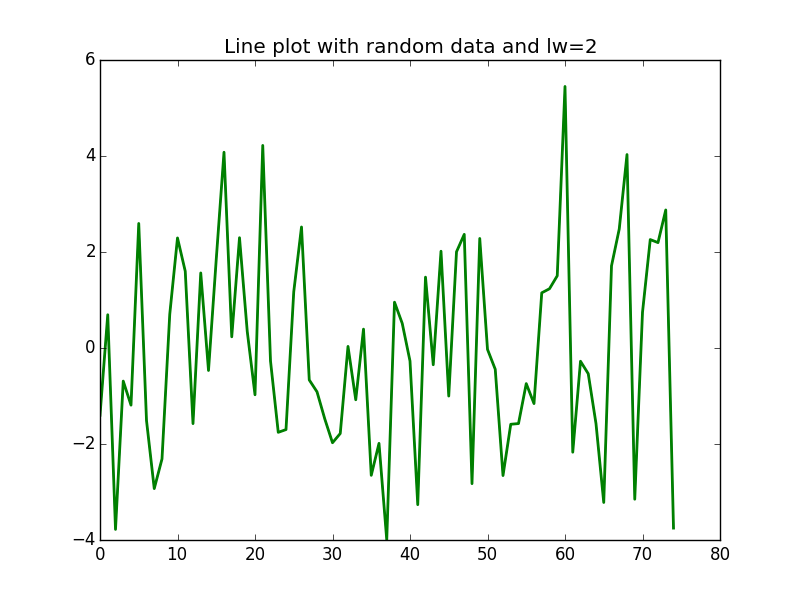
\includegraphics[width=\textwidth]{line_plot_good.png}
\end{subfigure}
\caption{Line Plot.  The left plot is plotted with \li{lw=1} whereas the right plot is plotted with \li{lw=2}.  Notice that the right plot is better because it is easier to see the line.} % Irrelevant for right here.
\label{fig:lineplot_bad}
\end{figure}

\begin{figure}[h]
\centering
\begin{subfigure}{.5\textwidth}
\centering
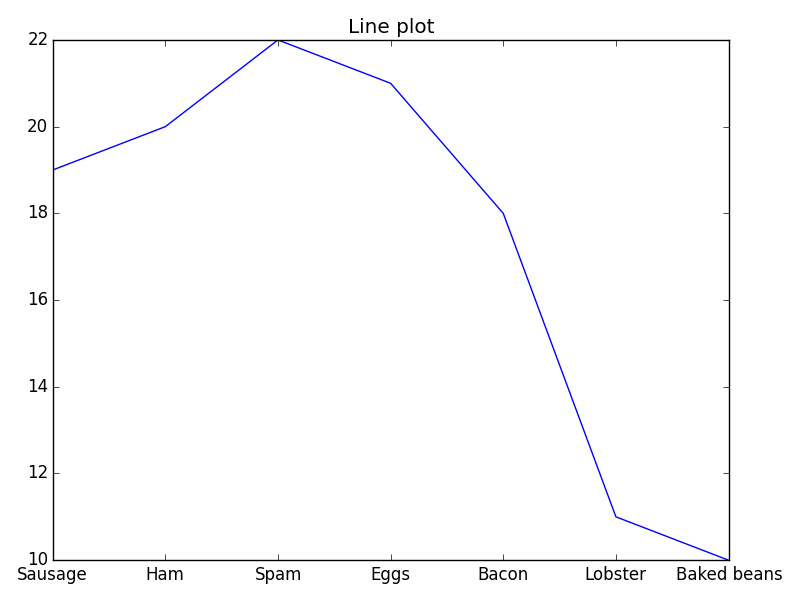
\includegraphics[width=\textwidth]{line_plot_bad_X.png}
\end{subfigure}
\caption{Line plot. Notice that this graph appears to show that the x-values are ordered. However, in reality, they are unordered. This is a bad practice and misrepresents the data.}
\label{fig:lineplotbadX}
\end{figure}
\end{comment}

\begin{comment} % MOVE BELOW.
\begin{figure}[h] % Choose an ethical scale and window.
\centering
\begin{subfigure}{.45\textwidth}
\centering
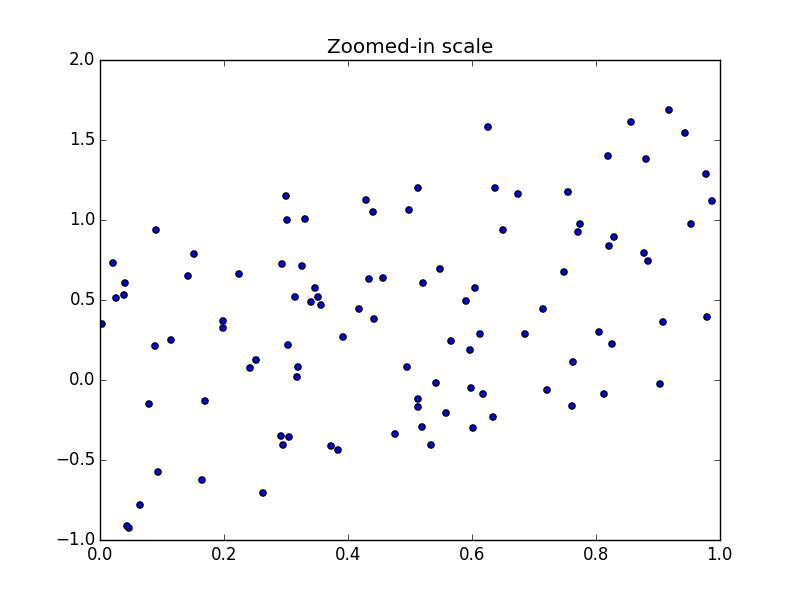
\includegraphics[width=\textwidth]{scale_scatter_zoomed_in.png}
\end{subfigure}
\begin{subfigure}{.45\textwidth}
\centering
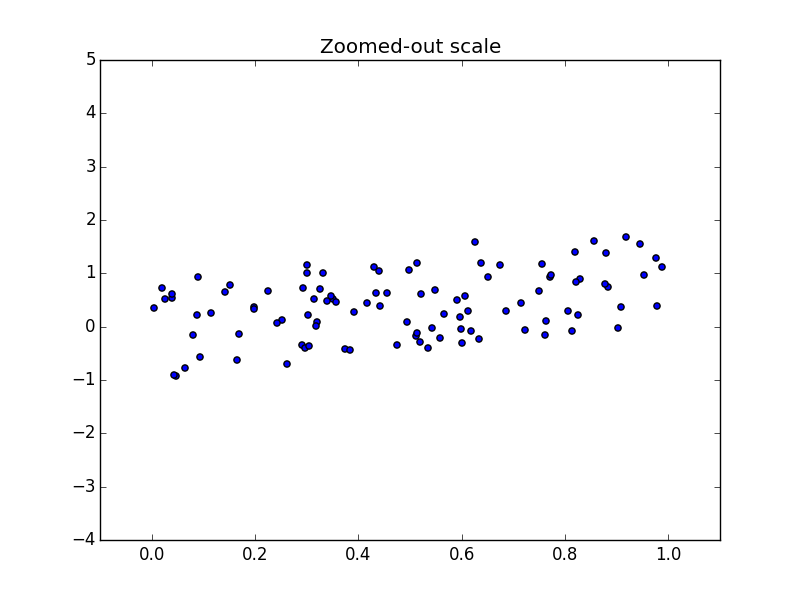
\includegraphics[width=\textwidth]{scale_scatter_zoomed_out.png}
\end{subfigure}
\caption{Scatter Plots. The data in both plots are the same but there appears to be a weaker
correlation in the first plot compared to the second.}
\label{fig:scatter_correlation}
\end{figure}
\end{comment}

\begin{comment}
\begin{figure}[h]
\centering
\begin{subfigure}{.45\textwidth}
\centering
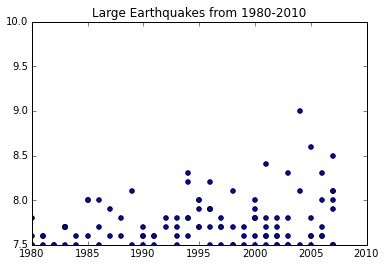
\includegraphics[width=\textwidth]{earthquake_zoomed.png}
\end{subfigure}
\begin{subfigure}{.45\textwidth}
\centering
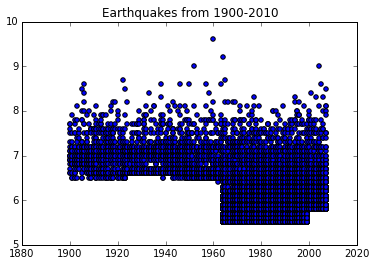
\includegraphics[width=\textwidth]{earthquake_data.png}
\end{subfigure}
\caption{USGS Earthquake data. The scatter plot on the left only plots earthquakes with
magnitude 7.5 or greater from 1980-2010 and appears to have a correlation.
However, the plot on the right shows all recorded earthquakes from 1900-2010 and shows that the correlation
is not a true correlation.}
\label{fig:scatterquake}
\end{figure}

Scatter plots may reveal insights other than correlation.
Consider Figure \ref{fig:scatterquake} which plots earthquake data from the United States Geological Survey (USGS).
The USGS data began including earthquakes with magnitude 6.5 or greater; this is clearly seen
in the scatter plot of the entire dataset.
Plots like this may also reveal errors in the dataset that are harder to detect in a table of values.
\end{comment}

\begin{comment}
\begin{figure}[h] % Bad visualization: earthquake data, year vs magnitude.
\captionsetup[subfigure]{justification=centering}
\centering
\begin{subfigure}{.5\textwidth}
    \centering
    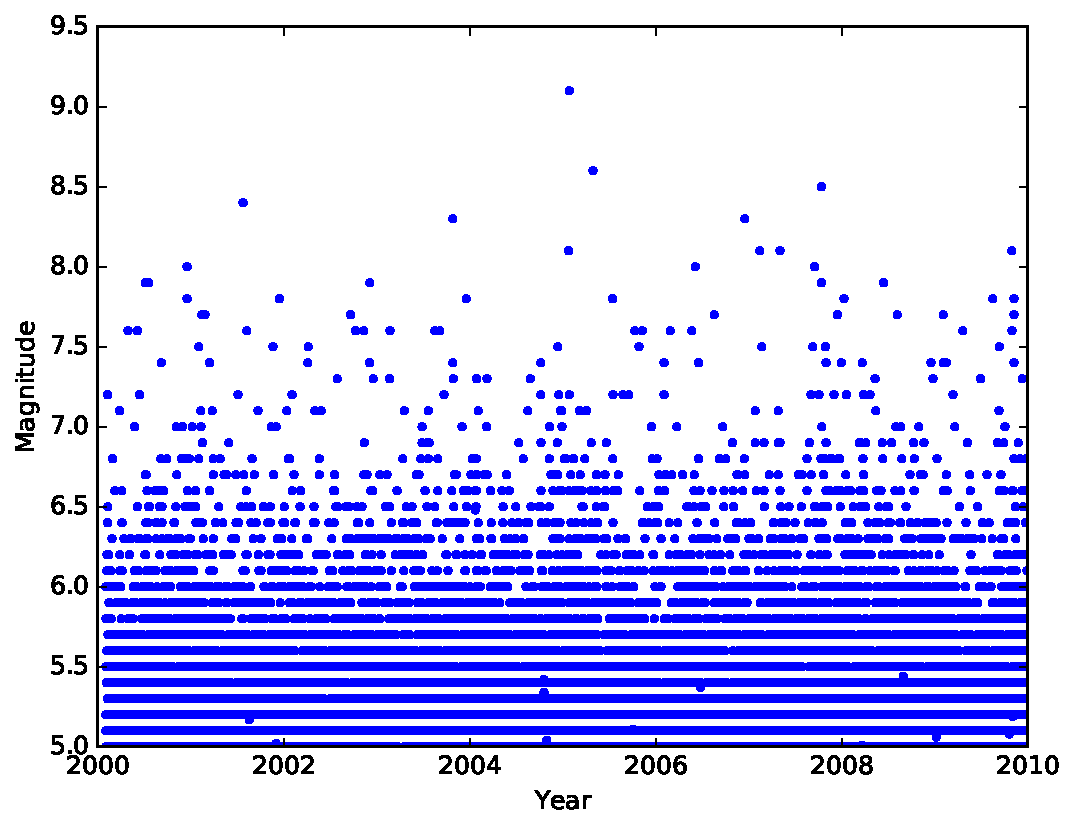
\includegraphics[width=\linewidth]{figures/earthquake_bad.pdf}
\end{subfigure}%
\begin{subfigure}{.5\textwidth}
    \centering
    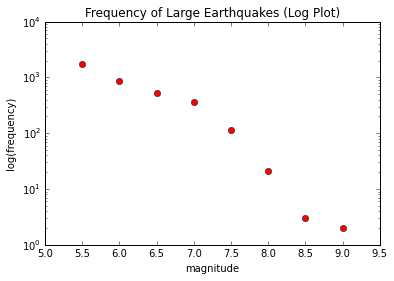
\includegraphics[width=\linewidth]{freq_earthquake_log.png}
\end{subfigure}
\caption{The left plot shows earthquakes of magnitudes 7.5 or higher over time. The right plot shows the frequencies of
different magnitudes. Note the scale of the y-axis is logarithmic.}
\label{fig:logexample}
\end{figure}
\end{comment}

\begin{comment} % This needs to go somewhere else.
Understanding a data set through visualizations is an iterative process.
Start with an initial visualization---usually a broad overview---and examine the data, then adjust the visualization or create other visualizations based on what you observe.
Ask the following questions as you search for insights:
\begin{enumerate}
\item Does the data make sense?
\item Would a different visualization communicate more information?
\item Would visualizing a subset of the data provide more information?
\item Would transforming the data reveal a hidden pattern?
\end{enumerate}
\end{comment}

As in any form of communication, integrity is important in data visualization.
Every visualization should be presented alongside all relevant information including who created it, where the data was obtained, how it was collected, whether it was cleaned or transformed, and whether there are conflicts of
interest or possible biases present.
Where appropriate, use words to carefully explain the insights represented
in the visualization.
These practices will help the reader correctly interpret the visualization.

\subsection*{Things to Avoid} % -----------------------------------------------

Some popular visualizations (pie charts, radar graphs, stacked bar charts and others) interfere with our ability to interpret the information they display.
For example, it is more difficult to detect differences in a pie chart than on a bar chart with the same data.
This is because differences in area are more difficult to detect than differences in length.
As a result, charts that depend on detecting variation in area will be less effective.
Instead, choose visualizations that compare the data to the a simple standard that is easy to understand and interpret.
Figures \ref{fig:pievsbar} and \ref{fig:stacked} are examples of poorly chosen visualizations.

\begin{figure} % Bad graphs.
\centering
\begin{subfigure}{.45\textwidth}
\centering
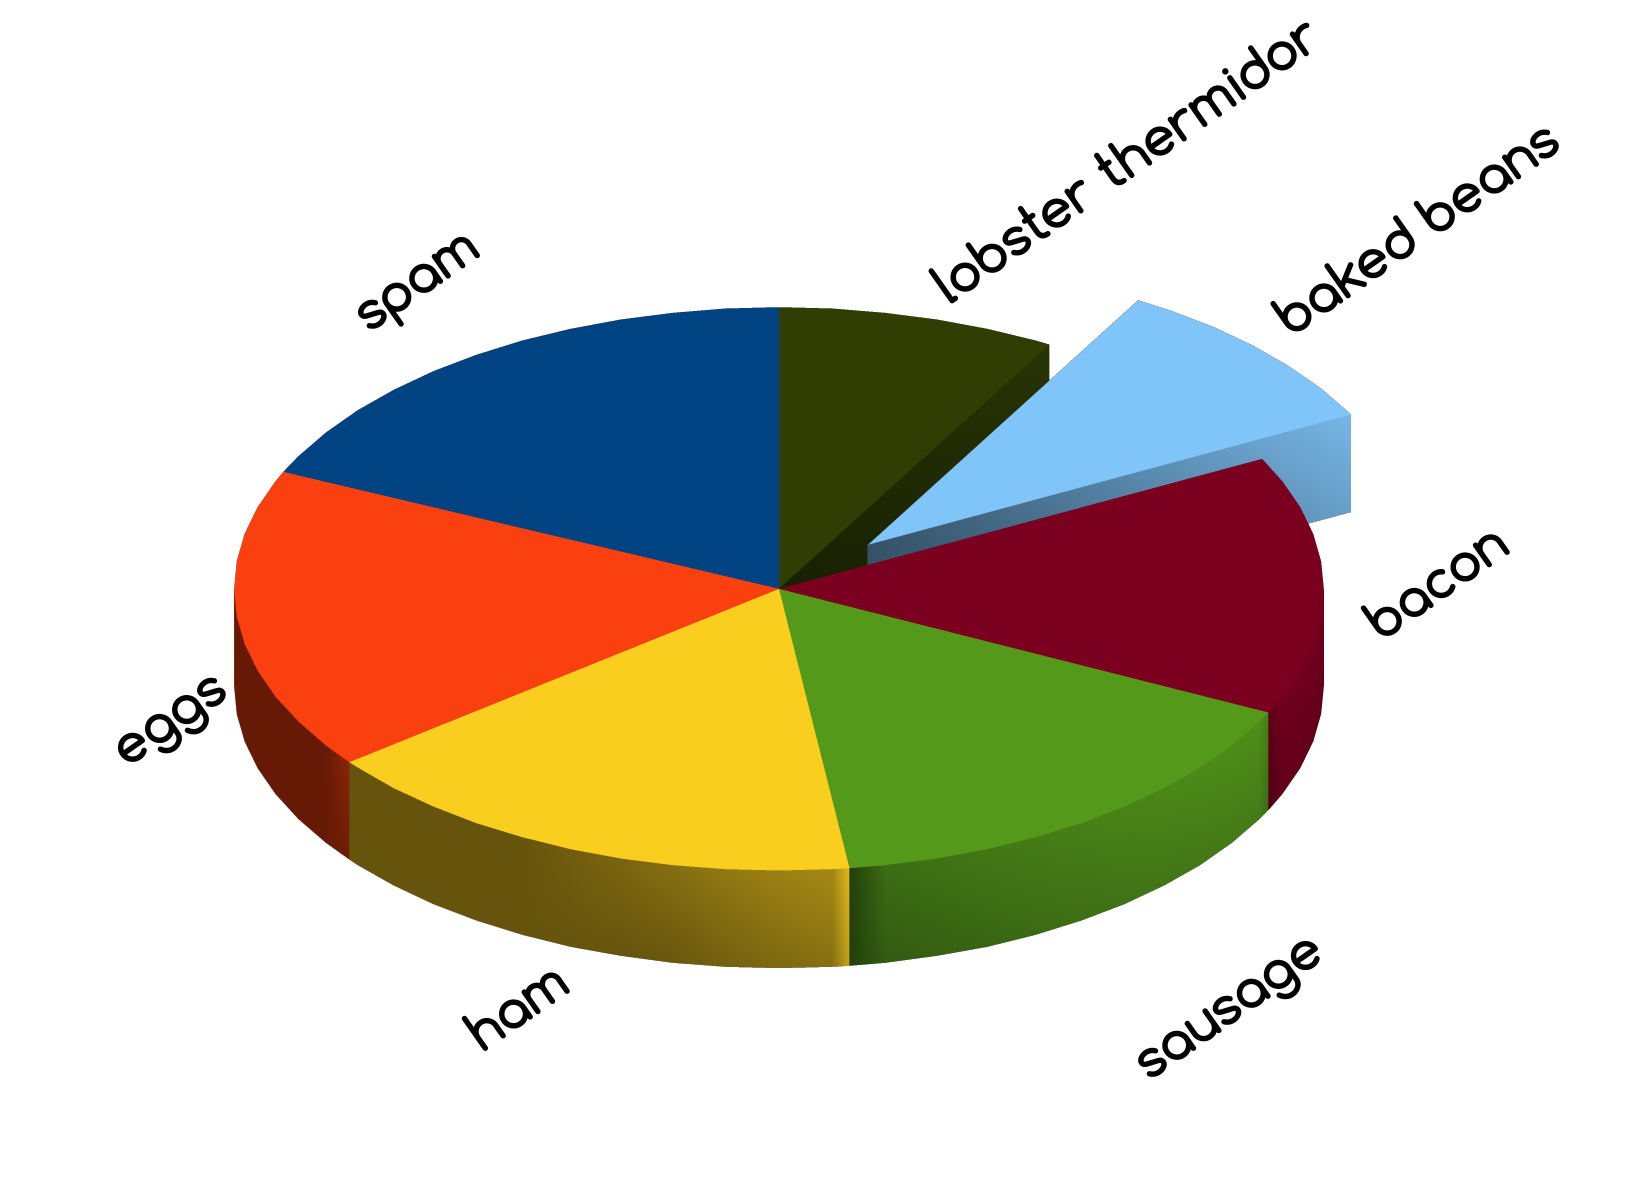
\includegraphics[width=\textwidth]{bad_pie_chart.png}
\end{subfigure}
\begin{subfigure}{.45\textwidth}
\centering
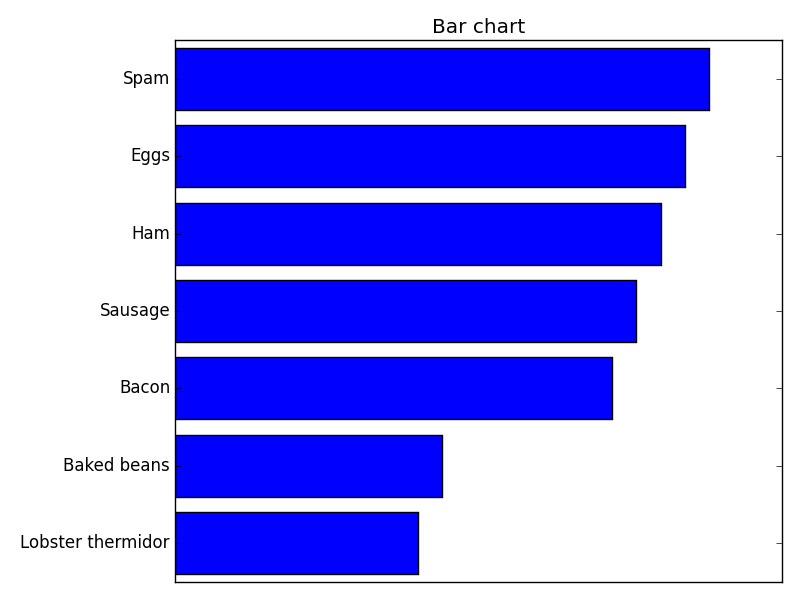
\includegraphics[width=\textwidth]{bar_chart_horizontal_sorted.png}
\end{subfigure}
\caption{A pie chart on the left that has been improved by a transformation into a bar chart on the right.}
\label{fig:pievsbar}
\end{figure}

\subsection*{Keep It Simple} % ------------------------------------------------

It may be tempting to stylize your visualization by adding icons and pictures or by making certain features
look 3D.  This is called chartjunk, a term coined by Edward Tufte. Chartjunk is anything in a plot that fails to add to or
misrepresents the data.  Avoid making visualizations that are overly fancy or cluttered with chartjunk. This
includes 3D effects (as in \ref{fig:pievsbar}), bad font choices, and unnecessary icons and pictures.
Visualizations are at their best when they are as simple as possible and allow the reader to easily
interpret the information being presented.

Reference lines can distract from the visualization (see Figure \ref{fig:histogram}).
For example, we can remove axis lines, tick marks, and bar lines
with the following code:

\begin{lstlisting}
# Get current axis instance
axis = plt.gca()

# Hide top and right spines
axis.spines['right'].set_visible(False)
axis.spines['top'].set_visible(False)

# Only show bottom and left tick marks
axis.yaxis.set_ticks_position('left')
axis.xaxis.set_ticks_position('bottom')
\end{lstlisting}

\begin{problem} % Problem: convert a pie chart to a horizontal bar chart.
Regraph the pie chart in Figure \ref{fig:pievsbar} as a horizontal bar chart using the follwing data.
Spam: 21, Eggs: 20, Ham: 22, Sausage: 21, Bacon: 20, Baked Beans: 11, Lobster Thermidor: 10
\end{problem}

\begin{figure} % Stacked v unstacked bar charts
\centering
\begin{subfigure}{.45\textwidth}
\centering
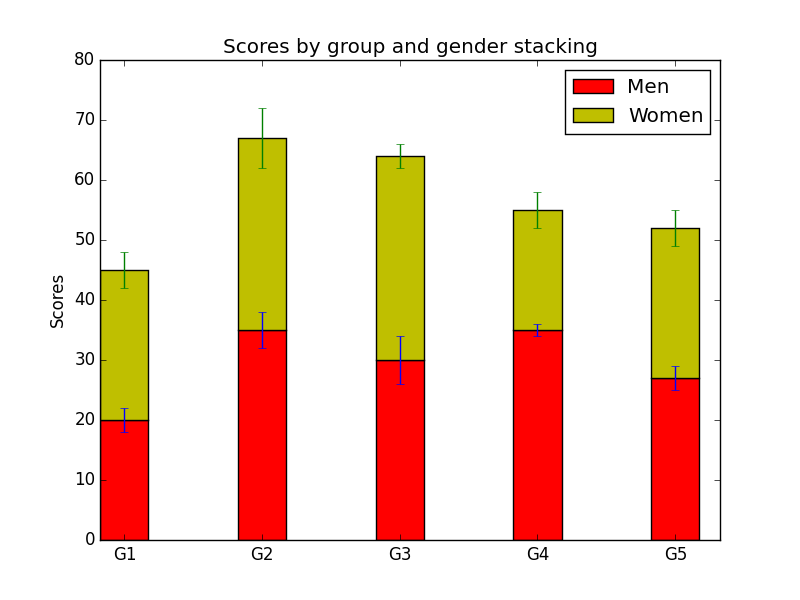
\includegraphics[width=\textwidth]{stackedbar.png}
\end{subfigure}
\begin{subfigure}{.45\textwidth}
\centering
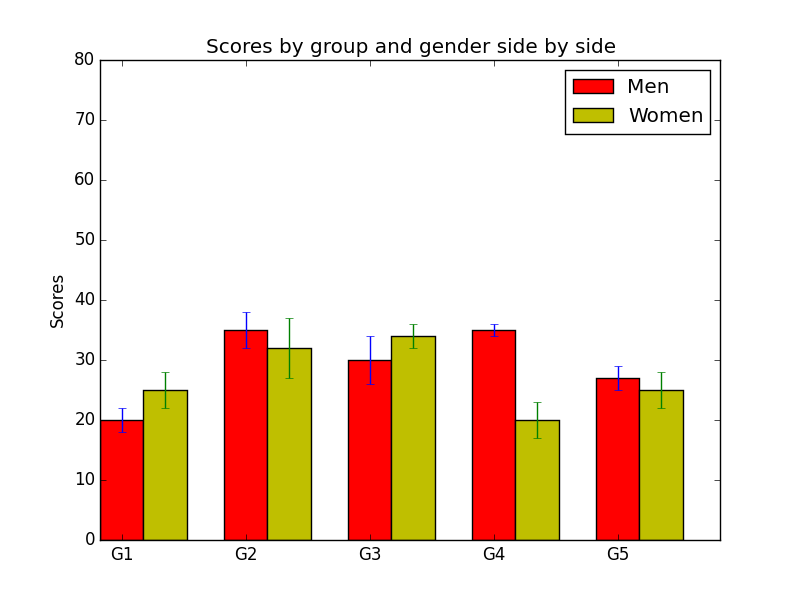
\includegraphics[width=\textwidth]{unstackedbar.png}
\end{subfigure}
\caption{Stacked Bar Chart. The relative values are harder to compare when stacked (left) instead of adjacent (right).}
\label{fig:stacked}
\end{figure}

\begin{comment}

\subsection*{Additional Material} % ===========================================

There are many software packages that facilitate the visual exploration of data.
One Python library is Glue (see \cite{glue}).

Some packages for making nicer looking plots include \li{Seaborn} and \li{prettyplotlib}.  TODO get refs

For more about visualization of data, we highly recommend the following books and websites:

% TODO get full refs for the follwoing

\begin{itemize}
    \item \emph{How to Lie with Statistics} by Darrell Huff (1954)
    \item \emph{Envisioning Information} by Edward Tufte
    \item \emph{The Visual Display of Quantitative Information} by Edward Tufte (2nd edition)
    \item \emph{Beautiful Evidence} by Edward Tufte
    \item \emph{Now you see it} by Stephen Few
    \item \url{http://www.informationisbeautiful.net/}
\end{itemize}

\end{comment}

%\noindent\emph{At their best, graphics are instruments for reasoning about quantitative information.} \small{---Edward Tufte}
% from the introduction of his book 'The Visual Display of Quantitative Information'

\begin{comment} % Move to 'Additional Material'.
\textbf{Bar Chart}: Best for small sets of discrete, one-dimensional, categorical data.
Usually, a horizontal bar chart is preferred over a vertical bar chart because it's harder to read vertical labels than horizontal labels.
Also, horizontal labels on a vertical bar chart may not fit on the graph well (see Figure \ref{fig:barchart}).

The data in a bar chart should be sorted in a logical way.
If the chart is being used to compare the values of different data points, it is best to sort by size; if the chart is being used to look up specific values, the labels should be sorted in a way that makes it easy to find specific values (for example, alphabetically).
Use \li{plt.bar()} or \li{plt.barh()} to create a bar chart in Matplotlib.

\begin{figure}[h] % Bar chart styles
\centering
\begin{subfigure}{.45\textwidth}
  \centering
  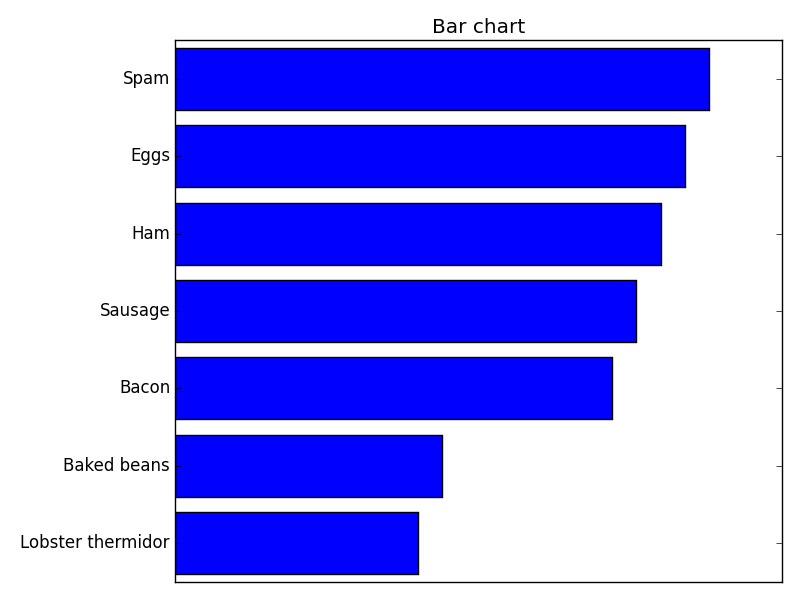
\includegraphics[width=\textwidth]{bar_chart_horizontal_sorted.png}
\end{subfigure}
\begin{subfigure}{.45\textwidth}
  \centering
  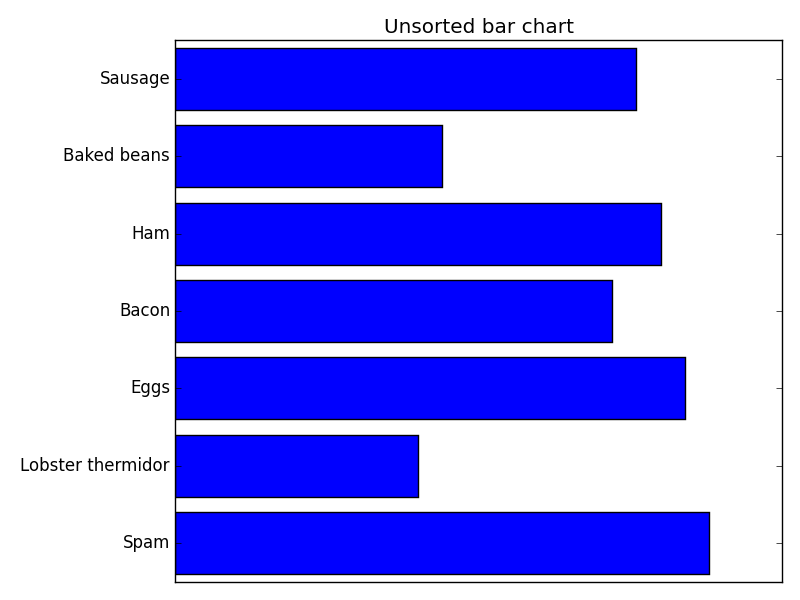
\includegraphics[width=\textwidth]{bar_chart_unsorted.png}
\end{subfigure}
\begin{subfigure}{.45\textwidth}
  \centering
  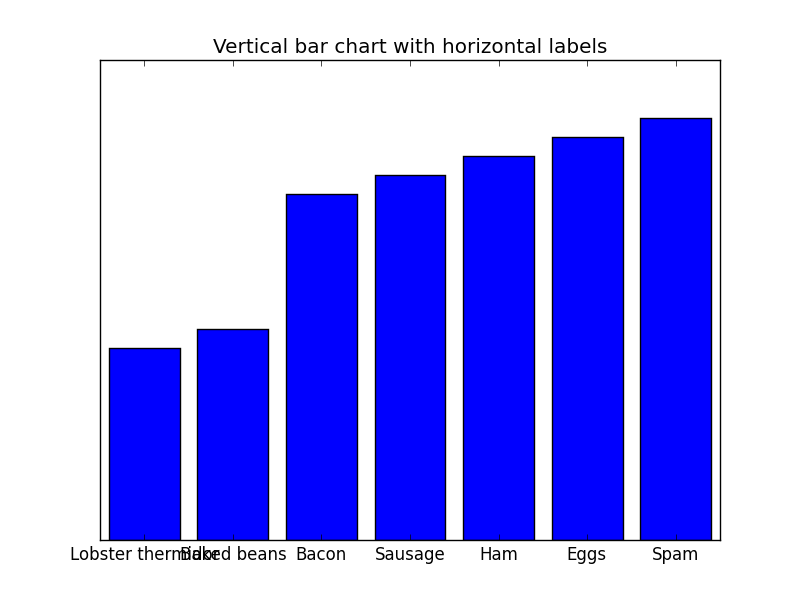
\includegraphics[width=\textwidth]{bar_chart_vertical_bars_horizontal_labels.png}
\end{subfigure}
\begin{subfigure}{.45\textwidth}
  \centering
  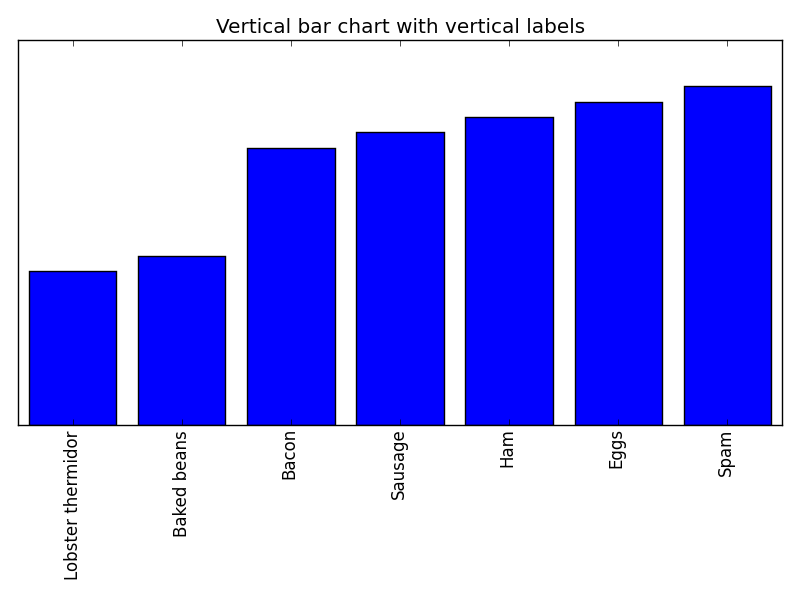
\includegraphics[width=\textwidth]{bar_chart_vertical_bars_vertical_labels.png}
\end{subfigure}

\caption{Bar Charts.
The example in the upper left is easier to use for comparison than the upper right, and easier to read than the bottom two charts.
The labels overlap in the bottom left and the labels are vertical in the bottom right, making them hard to read.}
\label{fig:barchart}
\end{figure}

\begin{lstlisting}
# This code created the top right bar chart.
labels = 'Spam', 'Eggs', 'Ham', 'Sausage', 'Bacon', 'Baked beans','Lobster thermidor'
val = [10, 11, 18, 19, 20, 21, 22]    # the bar lengths
pos = np.arange(7)+.5    # the bar centers on the y axis
plt.barh(pos,val, align='center')
plt.yticks(pos, labels[::-1])
plt.show()
\end{lstlisting}
\end{comment}

